\documentclass[a4paper]{article}
\usepackage[utf8]{inputenc}
\usepackage{csquotes}
\usepackage{tcolorbox}
\usepackage{verbatim}
\usepackage{a4wide,amssymb,epsfig,latexsym,multicol,array,hhline,fancyhdr}
\usepackage{vntex}
\usepackage{amsmath}
\usepackage{lastpage}
\usepackage[lined,boxed,commentsnumbered]{algorithm2e}
\usepackage{enumerate}
\usepackage{color}
\usepackage{graphicx}							% Standard graphics package
\usepackage{array}
\usepackage{tabularx, caption}
\usepackage{multirow}
\usepackage{multicol}
\usepackage{rotating}
\usepackage{graphics}
\usepackage{geometry}
\usepackage{setspace}
\usepackage{epsfig}
\usepackage{tikz}
\usepackage{listings}
\usepackage{color}
\usepackage[framemethod=tikz]{mdframed}

\usetikzlibrary{arrows,snakes,backgrounds}
\usepackage{hyperref}
\usepackage{indentfirst}
\hypersetup{urlcolor=blue,linkcolor=black,citecolor=black,colorlinks=true} 
%\usepackage{pstcol} 								% PSTricks with the standard color package

\newtheorem{theorem}{{\bf Định lý}}
\newtheorem{property}{{\bf Tính chất}}
\newtheorem{proposition}{{\bf Mệnh đề}}
\newtheorem{corollary}[proposition]{{\bf Hệ quả}}
\newtheorem{lemma}[proposition]{{\bf Bổ đề}}
\AtBeginDocument{\renewcommand*\refname{Tài liệu tham khảo}}

%\usepackage{fancyhdr}
\setlength{\headheight}{40pt}
\pagestyle{fancy}
\fancyhead{} % clear all header fields
\fancyhead[L]{
 \begin{tabular}{rl}
    \begin{picture}(25,15)(0,0)
    \put(0,-8){
\includegraphics[width=8mm, height=8mm]{hcmut.png}}
    %\put(0,-8){\epsfig{width=10mm,figure=hcmut.eps}}
   \end{picture}&
	%
\includegraphics[width=8mm, height=8mm]{hcmut.png} & %
	\begin{tabular}{l}
		\textbf{\bf \ttfamily Trường Đại Học Bách Khoa Tp.Hồ Chí Minh}\\
		\textbf{\bf \ttfamily Khoa Khoa Học và Kỹ Thuật Máy Tính}
	\end{tabular} 	
 \end{tabular}
}
\fancyhead[R]{
	\begin{tabular}{l}
		\tiny \bf \\
		\tiny \bf 
	\end{tabular}  }
\fancyfoot{} % clear all footer fields
\fancyfoot[L]{\scriptsize \ttfamily Bài tập lớn môn Mô hình hóa Toán học, Học kỳ 1, Năm học 2022-2023}
\fancyfoot[R]{\scriptsize \ttfamily Trang {\thepage}/\pageref{LastPage}}
\renewcommand{\headrulewidth}{0.3pt}
\renewcommand{\footrulewidth}{0.3pt}


%%%
\setcounter{secnumdepth}{4}
\setcounter{tocdepth}{3}
\makeatletter
\newcounter {subsubsubsection}[subsubsection]
\renewcommand\thesubsubsubsection{\thesubsubsection .\@alph\c@subsubsubsection}
\newcommand\subsubsubsection{\@startsection{subsubsubsection}{4}{\z@}%
                                     {-3.25ex\@plus -1ex \@minus -.2ex}%
                                     {1.5ex \@plus .2ex}%
                                     {\normalfont\normalsize\bfseries}}
\newcommand*\l@subsubsubsection{\@dottedtocline{3}{10.0em}{4.1em}}
\newcommand*{\subsubsubsectionmark}[1]{}
\makeatother
\definecolor{dkgreen}{rgb}{0,0.6,0}
\definecolor{gray}{rgb}{0.5,0.5,0.5}
\definecolor{mauve}{rgb}{0.58,0,0.82}

\lstset{frame=tb,
	language=python,
	aboveskip=3mm,
	belowskip=3mm,
	showstringspaces=false,
	columns=flexible,
	basicstyle={\small\ttfamily},
	numbers=none,
	numberstyle=\tiny\color{gray},
	keywordstyle=\color{blue},
	commentstyle=\color{dkgreen},
	stringstyle=\color{mauve},
	breaklines=true,
	breakatwhitespace=true,
	tabsize=3,
	numbers=left,
	stepnumber=1,
	numbersep=1pt,    
	firstnumber=1,
	numberfirstline=true,
         literate={ctth}{{$\delta \leftarrow \left\{ r_{i,j}\in W \right\}$}}1 {GX}{{$G_x$}}1
}

\begin{document}

\begin{titlepage}
\begin{center}
ĐẠI HỌC QUỐC GIA THÀNH PHỐ HỒ CHÍ MINH \\
TRƯỜNG ĐẠI HỌC BÁCH KHOA \\
KHOA KHOA HỌC - KỸ THUẬT MÁY TÍNH 
\end{center}

\vspace{1cm}

\begin{figure}[h!]
\begin{center}

\includegraphics[width=3cm]{hcmut.png}
\end{center}
\end{figure}

\vspace{1cm}


\begin{center}
\begin{tabular}{c}
\multicolumn{1}{l}{\textbf{{\Large MÔ HÌNH HÓA TOÁN HỌC (CO2011)}}}\\
~~\\
\hline
\\
\multicolumn{1}{l}{\textbf{{\Large Bài tập lớn}}}\\
\\
\textbf{{\Huge Stochastic Programming}}\\
\textbf{{\Huge and Applications}}\\
\\
\hline
\end{tabular}
\end{center}

\vspace{2cm}

\begin{table}[h]
\begin{tabular}{rrlr}
\hspace{5 cm} & GVHD: & Nguyễn Tiến Thịnh\\
& SV: & Lê Ngọc Vinh &2213964 \\
& & Phan Tuấn Kiệt   &2211771 \\
& & Dương Hải Lâm &2211807 \\
& & Nguyễn Tuấn Huy &2211253 \\
& & Nguyễn Phan Đình Huy &2211228 \\
\end{tabular}
\end{table}
\vspace{2cm}
\begin{center}
{\footnotesize TP. HỒ CHÍ MINH, THÁNG 12/2023}
\end{center}
\end{titlepage}


%\thispagestyle{empty}

\newpage
\tableofcontents
\newpage
\section{Cơ sở lí thuyết}

{\textbf{Mathematical Optimization} (Tối ưu toán học) là bài toán tìm nghiệm tốt nhất trong một tập các ứng viên thỏa mãn một tiêu chí nào đó. }

{Trong lập trình, khái niệm \textit{"tính không chắc chắn"} thường được liên kết với việc xử lý dữ liệu hoặc điều kiện mà không biết trước giá trị cụ thể hoặc kết quả chính xác. Điều này thường xảy ra khi chúng ta có các biến hoặc điều kiện phụ thuộc vào các yếu tố không biết hoặc có thể thay đổi trong quá trình thực thi chương trình.}
\subsection{Stochastic Programming}
{\textbf{Stochastic Programming} là bài toán tối ưu với các tham số ngẫu nhiên. Sử dụng chương trình nhằm mục đích tìm ra giá trị tối ưu cho các biến quyết định nhằm giảm thiểu các nguy cơ rủi ro và xem xét các tình huống có thể xảy ra của các biến ngẫu nhiên}

{Các loại mô hình:}
\begin{itemize}
    \item Mô hình two - stage: Mô hình cho ra quyết định trước khi sự không chắc chắn được phát hiện. Với ưu điểm là có thể giải quyết các bài toán quy hoạch ngẫu nhiên có các tham số ngẫu nhiên phụ thuộc lẫn nhau và có thể được sử dụng để giải quyết các bài toán quy hoạch ngẫu nhiên có các mục tiêu phức tạp, chẳng hạn như tối thiểu hóa rủi ro hoặc tối đa hóa xác suất đạt được mục tiêu. Ví dụ: Một công ty sản xuất có thể sử dụng mô hình two stage để xác định số lượng sản phẩm cần sản xuất để đáp ứng nhu cầu trong tương lai. Nhu cầu là một tham số ngẫu nhiên, vì nó phụ thuộc vào các yếu tố như thị trường, thời tiết. Trong giai đoạn 1, công ty có thể giả định nhu cầu là một giá trị xác định và giải quyết bài toán tối ưu hóa chắc chắn để xác định số lượng sản phẩm tối ưu cần sản xuất cho giá trị nhu cầu đó. Trong giai đoạn 2, nhu cầu thực tế sẽ được quan sát và công ty sẽ sản xuất số lượng sản phẩm thực tế dựa trên kết quả của giai đoạn 1.
    \item Mô hình multi - stage: Mô hình có nhiều giai đoạn quyết định và giải quyết không chắc chắn. Ưu điểm là nó có thể dẫn đến kết quả tối ưu hơn, vì các tham số ngẫu nhiên của bài toán được cập nhật ở mỗi giai đoạn. Ngoài ra, mô hình này cũng có thể được sử dụng để giải quyết các bài toán quy hoạch ngẫu nhiên có các tham số ngẫu nhiên phụ thuộc lẫn nhau. Ví dụ: Trong giai đoạn lập kế hoạch, một công ty có thể xác định nhu cầu như một giá trị cụ thể và giải quyết vấn đề tối ưu hóa chắc chắn để xác định số lượng sản xuất tối ưu  cho giá trị nhu cầu đó. Trong giai đoạn sản xuất, nhu cầu thực tế  được theo dõi và công ty sản xuất số lượng sản phẩm thực tế dựa trên kết quả của giai đoạn lập kế hoạch. Trong giai đoạn phân phối, công ty  phân phối số lượng sản phẩm thực tế dựa trên nhu cầu thực tế.
\end{itemize}
\subsection{Stochastic Linear Programming}
{\textit{Stochastic Linear Programming} là các bài toán quy hoạch tuyến tính (nghĩa là hàm mục tiêu của chúng là tuyến tính) trong đó một số dữ liệu có thể được coi là không chắc chắn.}

{Quy hoạch tuyến tính ngẫu nhiên (SLP) là sự tối ưu hóa sao cho Z đạt cực tiểu}
\[ Z = g(x) = f(x) = c^T . x \]
{Mà trong đó}

\[ A x = b  \ \& \   T x \geqslant h \]
\begin{itemize}
    \item x = ($x_1, x_2,...x_n$) là các biến quyết định
    \item A là ma trận tham số thực và b là vector tham số thực nhằm ràng buộc xác định (derterministic constraints), 
    \item  T, h là tập hợp các tham số ngầu nhiên xác định các ràng buộc xác suất 
\end{itemize}
\subsection{One - Stage Stochastic Linear Programming - No Recourse}
{\textit{One - Stage Stochastic linear programming - No recourse} là lập trình tối ưu hóa sao cho thỏa mãn z đạt cực tiểu:}
\[ Z = g(x) = f(x) = c^T . x=\sum_{j=1}^nc_jx_j \]
{Mà trong đó, LP($\alpha$) tham số hóa bởi vector ngẫu nhiên $\alpha$}

\[ A x = b  \ \& \   T x \geqslant h \]

{Với giả định rằng:}
\begin{itemize}
    \item Ma trận T = T($\alpha$) và vector h = h($\alpha$) thể hiện sự không nhất quán thông qua ràng buộc ngẫu nhiên (stochastic constrains)
    \[T(\alpha) x \geqslant h(\alpha) \iff \alpha_1 x_1 + ... + \alpha_n x_n \geqslant h(\alpha)\]
    \item Giá trị (T,h) là không xác định: Chúng không xác định trước khi một thực thể (instance) của mô hình xuất hiện, h($\alpha$) phụ thuộc duy nhất vào biến ngẫu nhiên $\alpha_j$.
    \item Sự không chắc chắn được biểu hòa bởi sự phân phối xác suất của các tham số ngẫu nhiên ($\alpha_j$)=$\alpha$ vì thế xác định quy hoạch tuyến tính là một trường hợp của quy hoạch tuyến tính ngẫu nhiên khi $\alpha_j$ là một hằng số
    \begin{itemize}
        \item Quyết định vấn đề khi vector x = ($x_1, x_2,...x_n$) $\in \chi$ của biến quyết định phải được tạo trước khi hiện thực hóa vector tham số $\alpha \in \Omega$ xác định được.
        \item Thông thường ra đặt giới hạn trên và giới hạn dưới thông qua 
        \[\chi = x \in \mathbb{R}^n: l \leqslant x \leqslant u \]
    \end{itemize}
\end{itemize}

{\textbf{Phương pháp tiếp cận}: Trong lập trình tham số ngẫu nhiên, ta tối ưu một số giả định và chân trị}
\begin{itemize}
    \item Giả định cơ bản (Fundamental assumotion) - Chúng ta đã biết phân phối xác suất chung của dữ liệu, do đó ta tieeos cận đầu tiên cung cấp LP ràng buộc xác suất.
    \item Phân tích tình huống (The Scenario Analysis)- không hoàn hảo nhưng hữu dụng, cách tiếp cận tình huống giả định rằng có một số lượng hữu hạn các quyết định mà tự nhiên có thể đưa ra (kết quả của sự ngẫu nhiên). Mỗi quyết định khả thi là scenario
\end{itemize}
\subsubsection{Sử dụng Chance constraint và Acceptable risk}
{Chúng ta có thể thay thế T(x) $\geq$ h với ràng buộc xác suất $\mathbb{P}$[T x $\geq$ h] $\geq p^2$ với mức độ đáng tin cậy p $\in$ (0.5, 1), (được đưa ra bởi người đưa ra vấn đề.)}

{Rủi ro cần được quan sát nếu định nghĩa được:}
\[\text{acceptable risk } r_x := \mathbb{P}[Not (Tx \ge h) = \mathbb{P}[Tx \le h] \le 1 - p\]

{Khi đó (1-p) là giá trị rủi ro tối đa có thể chấp nhận}

{Ràng buộc khả năng T x $\leq$ h nghĩa là rủi ro chấp nhận được $r_x$ bé hơn giá trị tối đa 1 - p $\in$ (0,1) }
\subsubsection{Dùng cho ràng buộc ngẫu nhiên T($\alpha$)x $\leq$ h($\alpha$)}
{ Sử dụng phân tích tình huống (Scenario analyst) T($\alpha$)x $\leq$ h($\alpha$)}
{Với mỗi scenario ($T^*;h^*$), s= 1, ...,S}, tối thiểu hóa phương trình: ${f(x) = c^T \cdot x;\ sao \ cho \ Ax = b, T^sx \le h^s}$

{Ưu điểm: Mỗi vấn đề scenario là một LP}

{Nhược điểm: Phân bố rời rạc khiến cho mô hình có thể lồi (mixed - integer LP)}
\subsection{Generic Stochastic Programming with Recourse}
{ Định nghĩa: Sự tối ưu 2-SP được mở rộng từ định nghĩa 1.3 }
\[ \min\limits_{x}{g(x)} \text{ với } g(x) = f(x) + E_\omega[v(x,\omega)]\]\\
{Trong đó:}
\begin{itemize}
    \item với $x = (x_1,x_2,\cdot\cdot\cdot,x_n)$ là các biến quyết định bước đầu tiên
    \item $f(x)$ có thể tuyến tính hoặc không, là một hàm của mục tiêu  g(x)
    \item Trung bình  $Q(x) := E_\omega[v(x, \omega)]$ của hàm
    \[v: \mathbb{R}^n \times \mathbb{R}^S \longrightarrow \mathbb{R}\]\\
    {dựa trên ảnh hưởng của các giả định $\omega$. Q(x) là giá trị tối ưu của bước 2}
    \[\min\limits_{y\in \mathbb{R}^p}{\mathbf{q \ y} | \ sao \ cho \ T \cdot x + W \cdot \mathbf{y} = h}\]
    \item Các vectơ $\alpha = \alpha(\omega)$ và y = y($\omega$) được đặt tên là các biến quyết định, điều chỉnh hoặc truy hồi, chỉ được biết sau thực nghiệm e
\end{itemize}

{Nói cách khác, ta cực tiểu hóa tổng chi phí dự kiến g(x)=f(x)+Q(x) thõa mãn}
\[W\cdot y(\omega) = h(\omega) - T(\omega) \cdot x\]

{Ở đây, $W$ được gọi là $m \times p$ ma trận recourse (recourse matrix), chúng ta bắt đầu với trường hợp đơn giản $m = 1$, $\mathbf{q}$ là vector đơn vị unit recourse, cùng chiều với $y$ và $y = y(\omega) \in \mathbb{R}^p.$}
\newpage
\textbf{Giải quyết vấn đề mô hình truy hồi}
\begin{itemize}
    \item Mục tiêu lớn g(x) của chúng ta được xây dựng từ f(x) và Q(x). Trong đó y là vector quyết định của một vấn đề Second stage Lp, giá trị y phụ thuộc vào thực tế của $(T,h) := (T(\omega),h(\omega))$ biến recourse $y(\omega) \sim$ với các biện pháp sửa lỗi, ví dụ như sử dụng nguồn lực sản xuất thay thế - alternative production resources (overtime...).
    \item Đo lường rủi ro định lượng: độ lệch h($\omega$) - T($\omega$) · x là phù hợp.
    \item Ở đây RỦI RO được mô tả bằng chi phí truy hồi dự kiến Q(x) của quyết định x.
    \item Mô hình cải cách thực tế: q và W đến từ đâu?
\end{itemize}
\subsection{Two - Stage Stochastic Linear Programming }
\subsubsection{Mô hình Two-Stage SLP with Recourse (dạng đơn giản)}
{Quy hoạch tuyến tính ngẫu nhiên hai giai đoạn có recourse (2-SLPWR), hoặc chính
xác hơn là với biện pháp penalize corrective, thường được mô tả như sau}
\[2-SLP:  \min\limits_{x \in X}{c^T \cdot x} + \min\limits_{y(\omega) \in Y}{E_\omega[q \cdot y]}\]

{Hay tổng quan hơn là:}
\[2-SLP:  \min\limits_{x \in X, y(\omega)\in Y}{E_\omega[c^T \cdot x + v(x, \omega)]}\]
{Với v(x,$\omega$):= q$\times$y sao cho}
\begin{itemize}
    \item $Ax = b$ First Stage Constraints
    \item $T(\omega) \cdot x + W \cdot y(\omega) = h(\omega)$ Second Stage Constraints
\end{itemize}
{Hay ngắn gọn hơn: $W \cdot y = h(\omega) - T(\omega) \cdot x$}

{Bài toán SLP này chỉ định 2-SP trước đó (1.4) cho mục tiêu cụ thể - một hàm mục tiêu ngẫu nhiên (random grand objective) cụ thể g(x) có :}
\begin{enumerate}
    \item Hàm f(x)xác định, là một hàm tuyến tính trong quá trình tính toán
    \item Hàm xác suất v(x,$\omega$) liên quan đến các scenarios 
\end{enumerate}

{y=y(x,$\omega) \in \mathbb{R}_+^p$ được gọi là biến hành động hồi quy (recourse action variable) cho quyết định $x$ và thực tế của $\omega$. Hành động hồi quy (recourse action) được xem như là các biện pháp sửa lỗi trong SLP}

{}
%##############################################################################################################################################################################################################################################################################################################################################################################################################################################################################################################################################################################################################################################################################################################################################################################################################################################
\section{Problem 1}
{Một hãng công nghiệp F sản xuất $n=8$ sản phẩm. Tổng cộng có $m=5$ linh kiện khác nhau được đặt hàng từ các nhà cung cấp bên thứ 3. Mỗi sản phẩm i cần $a_{ij}\geq 0$ linh kiện j với \textit{$i=1,...,8$} và $j=1,...,5$. Nhu cầu của các sản phẩm sẽ được biểu diễn bằng vector ngẫu nhiên $w=D=(D_1,D_2,...,D_8)$.}
\newpage
{\textbf{Giai đoạn thứ hai:}}

{Đối với một giá trị quan trắc $d=(d_1, d_2,..., d_n)$ của vector ngẫu nhiên D. Ta có thể tìm ra phương án sản xuất tốt nhất bằng cách giải bài toán SLP với các biến quyết định $z=(z_1, z_2,..., z_8)$ - số lượng đơn vị được sản xuất, biến quyết định khác $y=(y_1, y_2,..., y_n)$ - số lượng linh kiện còn lại trong kho.}

\[LSP: \underset{z,y}{min}~Z = \sum_{i=1}^{8}(l_i-q_i)z_i-\sum_{j=1}^{5}s_jy_j \tag{1} \]

{Trong đó $s_j<b_j$ (chi phí đặt hàng trước mỗi linh kiện j) và $x_j$, $j=1,...,5$ là số lượng linh kiện cần đặt hàng trước khi sản xuất sao cho}
\[
\left\{\begin{matrix}
$y_j=x_j- \sum \limits_{i=1}^{8}a_{ij}z_i,~ j=1,...5$ \\
$0 \leq z_i\leq d_i,~ i= 1,...,n;~ y_j \geq 0,~ j=1,...,5$
\end{matrix}\right.
\]
{Toàn bộ mô hình (của giai đoạn thứ hai) có thể được biểu diễn tương đương như sau:}
\[
MODEL=
\left\{\begin{matrix}
$min_{z,y}~Z=c^T. z-s^T. y$ \text{với } c = (c_i:=l_i-q_i) \\
y = x - A^Tz, \text{trong đó } A = [a_{ij}] \text{ là ma trận $8 \times 5$} \\
0 \leq z \leq d,~y \geq 0.
\end{matrix}\right.
\]
{Lời giải của bài toán này, tức là vector $z, y$ phụ thuộc và việc thực hiện $d$ của nhu cầu ngẫu nhiên $w=D$ cũng như quyết định giai đoạn thứ nhất $x=(x_1, x_2,..., x_5)$.}

{\textbf{Giai đoạn thứ nhất:}}

{Toàn bộ mô hình 2-SLPWR dựa trên một quy tắc phổ biến \textit{sản xuất} \leq \textit{nhu cầu}}

{Bây giờ, làm theo cách tiếp cận dựa trên phân phối, ta đặt $Q(x):=E[Z(z,y)]=E_w[x,w]$ biểu thị giá trị tối ưu của vấn đề (1). Ký hiệu $b=(b_1, b_2,..., b_5)$ được xây dựng theo chi phí đặt hàng trước $b_j$ trên mỗi linh kiện $j$ (trước khi biết nhu cầu). Các đại lượng $x_j$ được xác định từ bài toán tối ưu sau}

\[
min~g(x,y,z) = b^T.~x + Q(x) = b^T.~x + E[Z(x)] \tag{2}
\]

{trong đó $Q(x)=E_w[Z]=\sum \limits_{i=1}^{n}p_ic_iz_i$ liên quan đến phân bố xác suất của $w=D$.}

{Phần đầu tiên của hàm mục tiêu biểu diễn chi phí đặt hàng trước và $x$. Ngược lại, phần thứ hai thể hiện chi phí dự kiến của kế hoạch sản xuất tối ưu (1), được xác định bởi số lượng đặt hàng $z$ được cập nhật, đã sử dụng nhu cầu ngẫu nhiên $D=d$ với mật độ của chúng.}

{\textbf{CÁCH GIẢI QUYẾT}}

\begin{itemize}
    \item {Các biến quyết định bao gồm các vector $x,y \in \mathbb{R}^5$ và $z \in \mathbb{R}^8$}
    \item {Sau khi quan sát thấy nhu cầu $D$, nhà sản xuất có thể quyết định phần nào của nhu cầu sẽ được đáp ứng để không vượt quá số linh kiện có sẵn. Chi phí bổ sung là $l_i$, để đáp ứng một đơn vị nhu cầu cho sản phẩm $i$, và giá bán của sản phẩm là $q_i$ }
    \item {Sau khi biết được nhu cầu $D$, ta xác định số lượng sản phẩm cần sản xuất. Các linh kiện không sử dụng sẽ bán thu được số tiền $s_j$, cho vector $s=(s_1, s_2,..., s_m)$}
\end{itemize}
\newpage
{\textbf{Ý TƯỞNG: }}{Bằng cách sử dụng GAMSPY:}
\begin{enumerate}
    \item[] {Đầu tiên ta tạo biến 1 Container để chứa các symbols của mô hình.}
    
    \begin{tcolorbox}[colback=blue!5!white,colframe=blue!75!black]
        \begin{verbatim}
    model = Container()
        \end{verbatim}
    \end{tcolorbox}
    \item[] {Ta tạo i, j, k lần lượt là các Set để chứa các products, parts và scenarios.}
    \begin{tcolorbox}[colback=blue!5!white,colframe=blue!75!black]
    \begin{verbatim}
    i = Set(container = model, name = 'i',
                description = 'products', records = products)
    j = Set(container = model, name = 'j', 
                description = 'parts', records = parts)
    k = Set(container = model, name = 'k',
                description = 'scenarios', records = scenarios)
    \end{verbatim}
    \end{tcolorbox}
    \item[] {Tạo các biến tham số A, l, q, b, s, d, p là các biến tham số (Parameter).}
    \begin{tcolorbox}[colback=blue!5!white,colframe=blue!75!black]
    \begin{verbatim}
A = Parameter(container = model, name = 'A', domain = [i, j],
        description = 'Requirements', 
            records = rqmts.reset_index())
l = Parameter(container = model, name = 'l', domain = [i],
        description = 'l_i := additional cost to satify a unit of 
        demand for product i',
            records = l.reset_index())
q = Parameter(container = model, name = 'q', domain = [i],
        description = 'q_i := unit selling price of product i',
            records = q.reset_index())
b = Parameter(container = model, name = 'b', domain = [j],
        description = 'b_j := cost per unit of part j', 
            records = b.reset_index())
s = Parameter(container = model, name = 's', domain = [j],
        description = 's_j := salvage values', 
            records = s.reset_index())
d = Parameter(container = model, name = 'd', domain = [i, k], 
        description = 'Demands', 
            records = demands.reset_index())
p = Parameter(container = model, name = 'p', domain = [k], 
        description = 'Density',
            records = density.reset_index())
    \end{verbatim}
    \end{tcolorbox}
    \newpage
    \item[] {Tạo x, y, z là các Variable, kiểu là số nguyên (INTEGER). x có domain là $j$, y có domain là $\{j,k\}$, z có domain là $\{i,k\}$}
    \begin{tcolorbox}[colback=blue!5!white,colframe=blue!75!black]
    \begin{verbatim}
x = Variable(container = model, name = 'x', type = 'INTEGER', 
        domain = [j], description =
            'x_j := parts to be ordered (1st stage decision)')
y = Variable(container = model, name = 'y', type = 'INTEGER',
        domain = [j, k], description = 
            'y_j := Parts left in inventory')
z = Variable(container = model, name = 'z', type = 'INTEGER',
        domain = [i, k], description = 
            'z_i := number unit of part j produced')
    \end{verbatim}
    \end{tcolorbox}
    \item[] {Từ các Parameter và các Variable đã tạo, ta khai báo và định nghĩa các Equation là các constraint của bài toán.}
    \begin{tcolorbox}[colback=blue!5!white,colframe=blue!75!black]
    \begin{verbatim}
eq1 = Equation(container = model, name = 'eq1', domain = [j, k])
eq1[j, k] = y[j, k] == x[j] - Sum(domain = [i], 
                                    expression = A[i, j] * z[i, k])
eq2 = Equation(container = model, name = 'eq2', domain = [j])
eq2[j] = x[j] >= 0
eq3 = Equation(container = model, name = 'eq3', domain = [j, k])
eq3[j, k] = y[j, k] >= 0
eq4 = Equation(container = model, name = 'eq4', domain = [i, k])
eq4[i, k] = z[i, k] >= 0
eq5 = Equation(container = model, name = 'eq5', domain = [i, k])
eq5[i, k] = z[i, k] <= d[i, k]
    \end{verbatim}
    \end{tcolorbox}
    \item[] {Sau đó ta tạo Model. Giải bài toán, chúng ta được giá trị tối ưu.}
    \begin{tcolorbox}[colback=blue!5!white,colframe=blue!75!black]
    \begin{verbatim}
problem1 = Model(container = model, name = 'Problem_1', 
    problem = 'MIP', sense = Sense.MIN, 
        equations = model.getEquations(), objective = obj)
    \end{verbatim}
    \end{tcolorbox}
\end{enumerate}
\newpage
\begin{figure}[h]
  \centering
  \subfigure{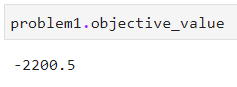
\includegraphics[width=0.45\linewidth]{obj_value.png}}
  \hfill
  \subfigure{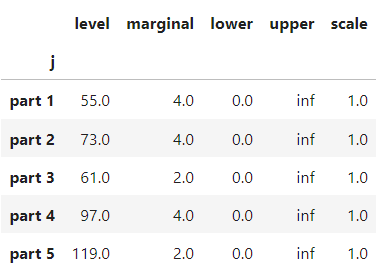
\includegraphics[width=0.5\linewidth]{x_records.png}}
  \hfill
  \medskip
  \subfigure{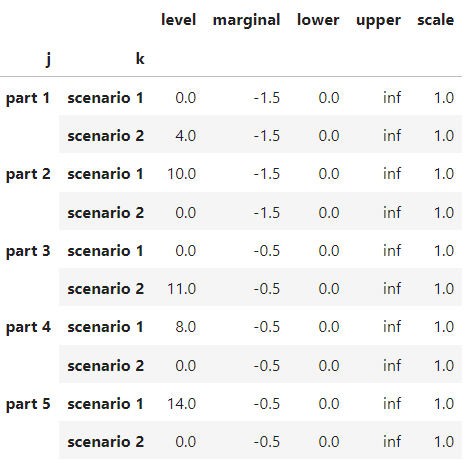
\includegraphics[width=0.5\linewidth]{y_records.png}}
   \hfill
  \subfigure{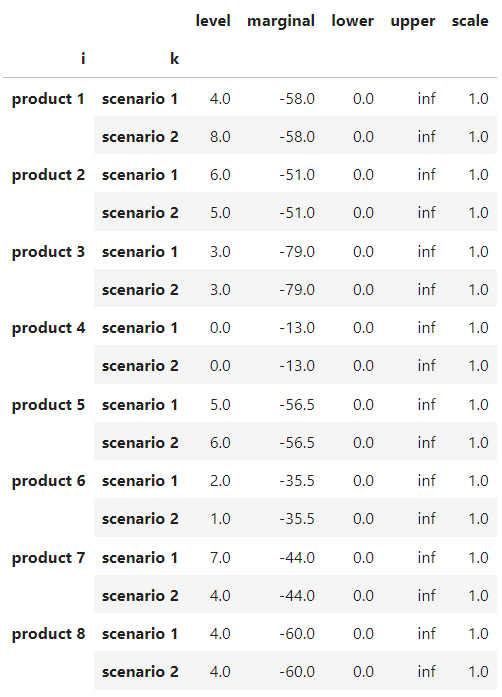
\includegraphics[width=0.45\linewidth]{z_records.png}} 
  \caption{Giá trị tối ưu tại $x, y, z$}
\end{figure}
\newpage
%#########################################################
\section{Problem 2}
\subsection{Tổng quan về bài toán Two-Stage Stochastic Evacuation Planning}
\subsubsection{Mô tả bài toán Two-Stages Stochastic Evacuation Planning. }
{Giả sử người ở vùng bị thảm họa nhận được cảnh báo về động đất và bắt đầu sơ tán đến nơi an toàn bằng xe của mình. Trong quá trình sơ tán (sau khi nhận được cảnh báo động đất) được cập nhật thông tin chính xác về trận động đất thông qua đài, thời sự, tin nhắn, (communication tools). Thời điểm cập nhật thông tin là threshold (T).}
\begin{enumerate}
    \item[-] {Bắt đầu sơ tán, di chuyển khi chưa biết chính xác phạm vi và mức độ ảnh hưởng chính xác của động đất. (Phụ thuộc vào một số tình huống thiệt hại).}
    \item[-] {Quá trình sơ tán được chia thành 2 giai đoạn theo thời gian thu thập thông tin:}
    \begin{enumerate}
        \item[+] {Giai đoạn 1: Trước khi nhận được thông tin chính xác về tình trạng đường đi thì đi theo kế hoạch ban đầu (priori evacuation). }
        \item[+] {Giai đoạn 2: Sau khi nhận được thông tin thì thay đổi đường đi cho phù hợp.} 
    \end{enumerate}
\end{enumerate}
 \(\Rightarrow\) {Mục tiêu là lập ra kế hoạch sơ tán trong giai đoạn 1 để có thể ứng phó với các tình huống phát sinh trong giai đoạn 2.}

 {Ví dụ: Two-Stage Stochastic Evacuation Planning Problem}
 \begin{figure}[h]
     \centering
     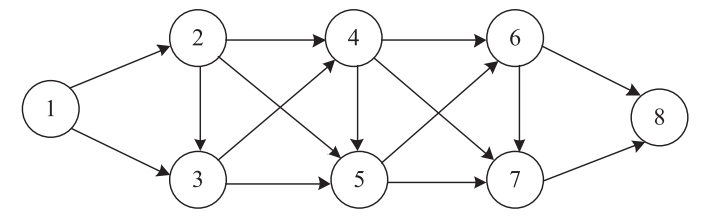
\includegraphics[scale=0.7]{road_network.png}
     \caption{An Illustrative Evacuation Road Network}
     \label{fig:enter-label}
 \end{figure}
 
{Kế hoạch ban đầu (priori evacuation):}
\begin{center}
 $a, b: 1-2-3-4-6-8$\\
 $c, d: 1-3-5-6-7-8$
\end{center}

{Kịch bản 1:}
 \begin{center}
 $a, b: 1-2-3-4-7-8$\\
 $c, d: 1-3-5-6-8$
 \end{center}

{Kịch bản 2:}
\begin{center}
$a, b: 1-2-3-4-6-8$ \\
$c: 1-3-5-6-8$ \\
$d: 1-3-5-6-7-8$
\end{center}
\begin{figure}[h]
    \centering
    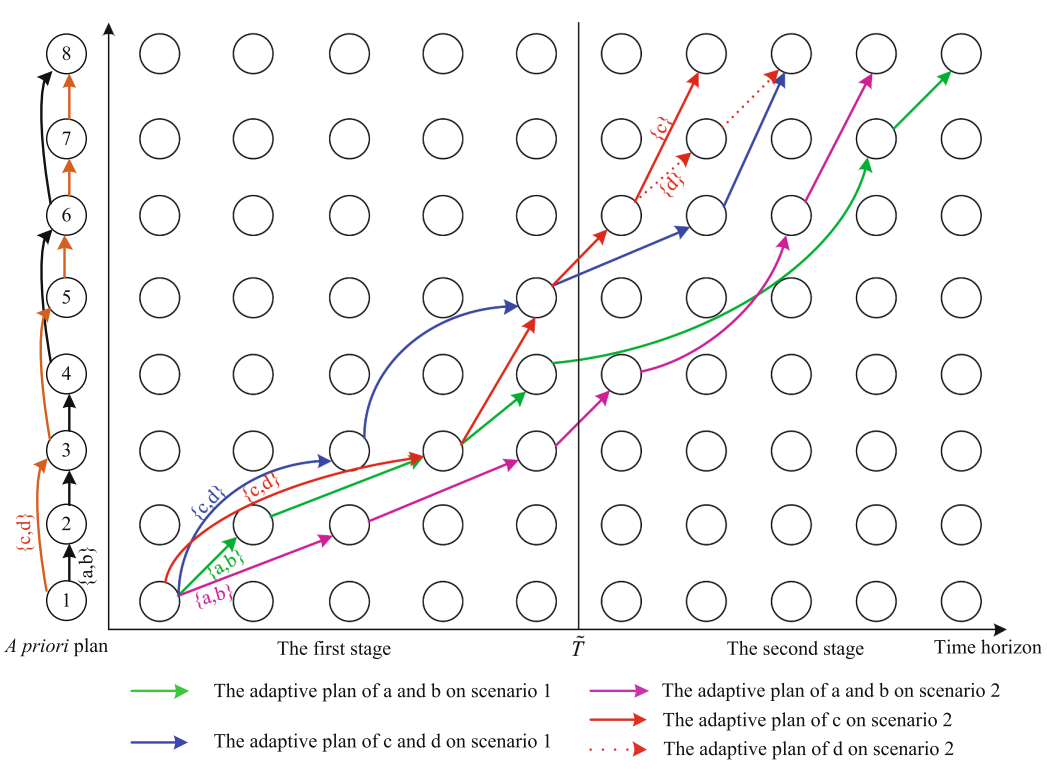
\includegraphics[scale=0.65]{time_dependent_network.png}
    \caption{Two-stage stochastic evacuation plan in time-dependent network.}
    \label{fig:enter-label}
\end{figure}

{Quá trình sơ tán được biểu diễn như trên. Trước threshold (T) đường đi trong các kịch b ản giống như đường đi trong kế hoạch ban đầu (priori evacuation). Sau threshold (T) đường đi tương ứng từng kịch bản sẽ khác với đường đi trong kế hoạch ban đầu (priori evacuation). }
\subsubsection{Chuyển đổi đồ thị một nguồn, một đích (Supersource và Supersink)}
{Trong bài toán sơ tán 2 giai đoạn có nhiều hơn 1 nguồn và 1 đích đến nên cần chuyển về thành 1 nguồn và 1 đích đến. }
\begin{enumerate}
    \item[-] {Với đồ thị không phụ thuộc thời gian}
    \begin{figure}[h]
        \centering
        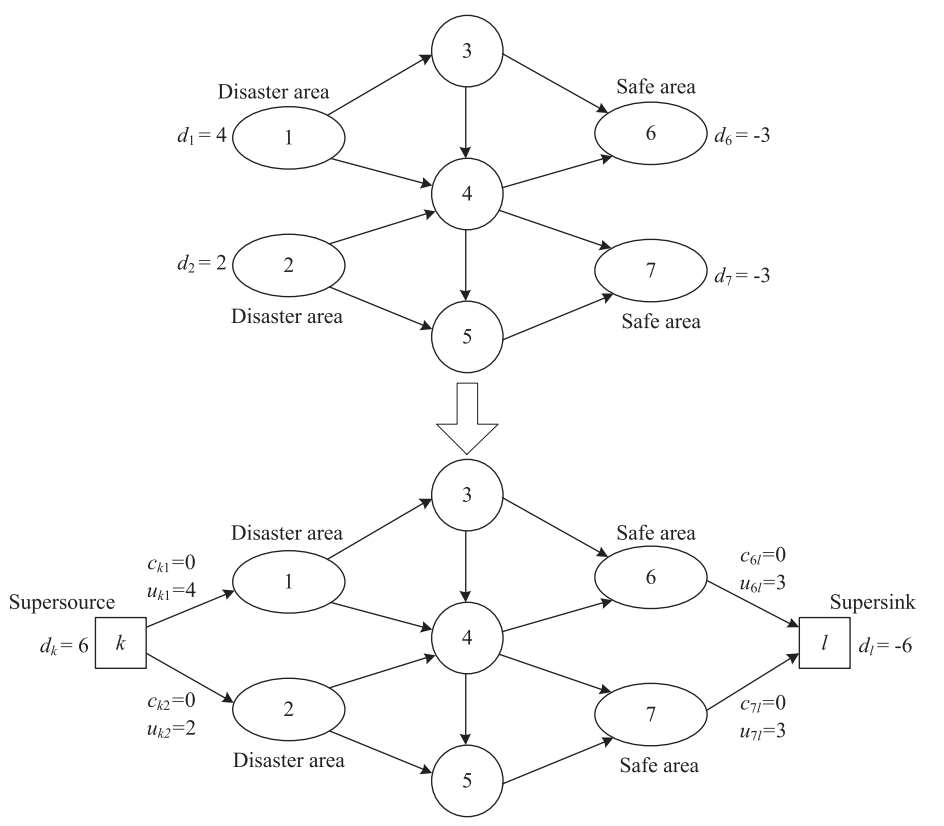
\includegraphics[scale=0.6]{physical_network.png}
        \caption{Supersource and Supersink conversion example in physical network.}
        \label{fig:enter-label}
    \end{figure}
    \\
    {Tạo thêm 1 node k (supersource): cạnh nối từ k đến các source cũ có cost (cki = 0), capacity (uki = di) do đó dk = Tổng di. (i: source, di: demand của từng source, dk: demand của supersource). Tương tự cho supersink.}
    \item[-] {Với đồ thị phụ thuộc thời gian}
    \begin{figure}[h]
        \centering
        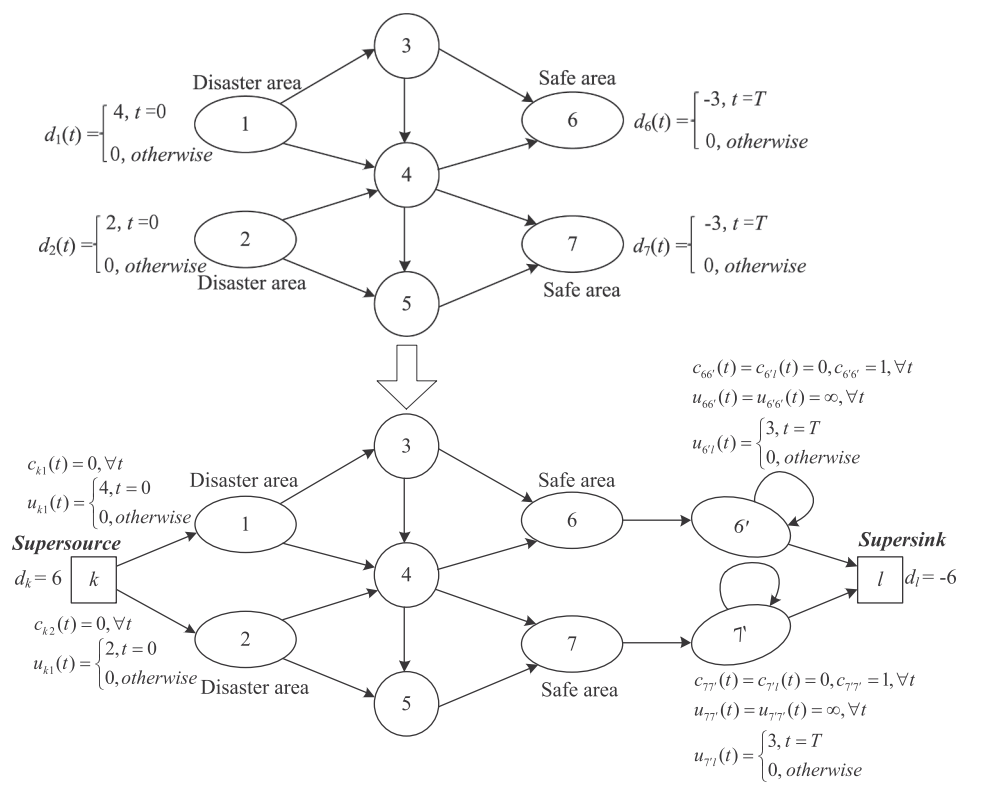
\includegraphics[scale=0.6]{time_dependent_1.png}
        \caption{Supersource and supersink conversion example in time-dependent network.}
        \label{fig:enter-label}
    \end{figure}
\end{enumerate}
{Supersource k: }
\begin{enumerate}
    \item[] {$c_{ki}$ luôn bằng 0}
    \item[] {$u_{ki} = d_i$ tại thời điểm bắt đầu, tất cả thời điểm khác bằng 0}
\end{enumerate}
{Supersink l: Vì thời gian đến sink của các đường đi khác nhau có thể khác nhau nên thêm 1 node copy j’ của sink j ban đầu. Thêm một vòng lặp vào j’}
\begin{enumerate}
    \item[] {$c_{jj’} = c_{j’l}$ luôn bằng 0, $c_{j’j’}$ luôn bằng 1}
    \item[] {$u_{jj’} = u_{j’j’}$ bằng vô cùng}
    \item[] {$u_{j’l} = d_j$ tại thời điểm T, tất cả thời điểm khác bằng 0} 
\end{enumerate}
\subsubsection{Giải quyết bài toán bằng Min-Cost-Flow Problem}
{Xem quá trình di chuyển người dân từ nơi nguy hiểm đến nơi an toàn như một min-cost flow problem với thời gian di chuyển (travel times) và sức chứa của đường (capacities) là ngẫu nhiên.}

{Mục tiêu là tìm lời giải của min-cost flow problem trong capacity-cost network $G(V, A, C, U, D)$}
\begin{enumerate}
    \item[] {$V$ là tập hợp các đỉnh (thành phố), }
	\item[]	{$A$ là tập hợp các cạnh (đường đi) với travel time và capacity ngẫu nhiên, }
	\item[]	{$C(i, j)$ là travel time trên cạnh $(i, j)$ thuộc A, kí hiệu $c_{ij}$,}
	\item[] {$U(i, j)$ là capacity trên cạnh $(i, j)$ thuộc A, kí hiệu $u_{ij}$,}
	\item[] {$D(i)$ là flow tại đỉnh $I$ thuộc $V$, kí hiệu $d_i$,}
\end{enumerate}
{Thời gian di chuyển (travel time) trên mỗi cạnh là không đổi. Sources tương đương với vùng nguy hiểm. Sinks tương đương với vùng an toàn.}

{Mô hình này khác với min-cost flow problem tổng quát. Cụ thể giai đoạn 1 và giai đoạn 2 xảy ra trong khoảng thời gian khác nhau trong cùng một mạng lưới sơ tán. Giai đoạn 1 thì travel times và capacities chỉ được biết theo xác suất, nhưng vẫn phải di chuyển người dân từ source đến các đỉnh khác trước khi nhận được thông tin về travel times và capacities thực tế sau threshold (T). Giai đoạn 2 thì xác định được kế hoạch sơ tán với travel times and capaticies cụ thể. Có thể kế hoạch sơ tán trong giai đoạn 1 không phù hợp với tình hình thực tế trong giai đoạn 2. Trong trường hợp này, hàm mục tiêu (objective function) sẽ bao gồm chi phí phạt (punish costs) và giá trị kì vọng của giai đoạn 2.}
\subsubsection{Xây dựng mô hình bài toán Two-stage stochastic evacuation planning. }
{Các kí hiệu}
\begin{figure}[h]
    \centering
    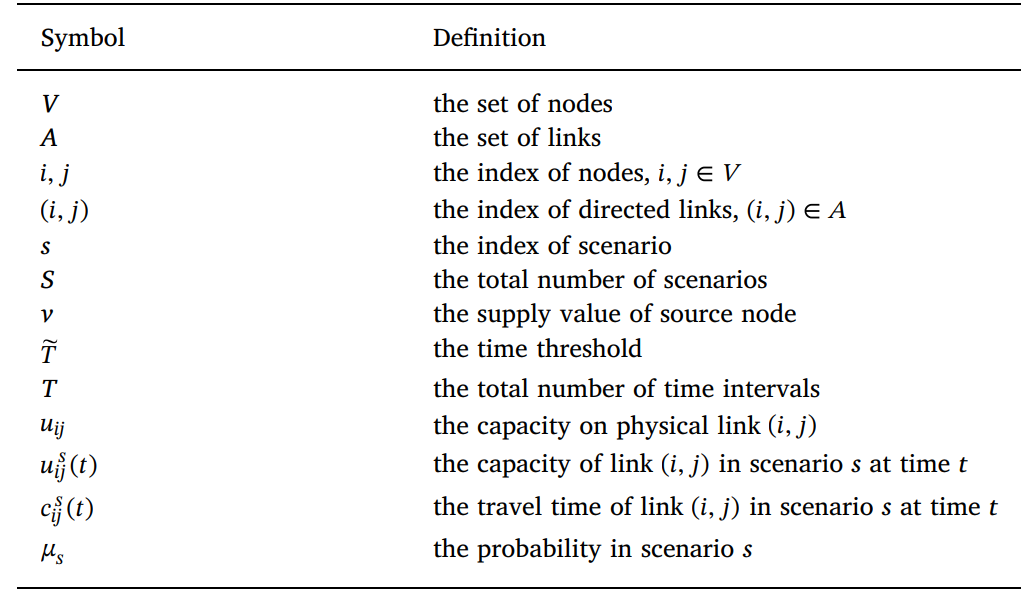
\includegraphics[scale=0.5]{table_1.png}
    \caption{Subscripts and Parameters Used in Mathematical Formulation.}
    \label{fig:enter-label}
\end{figure}
\newpage
{Decision variables}
\begin{enumerate}
    \item[] {Giai đoạn 1: $x_{ij}$ đại diện cho flow trên cạnh $(i, j)$.}
    \item[] {Giai đoạn 2: $y_{ij}^s(t)$ đại diện cho flow trên cạnh $(i, j)$ trong kịch bản $s$ tại thời điểm $t$.}   
\end{enumerate}

{System constraints}
\begin{enumerate}
    \item[] {Giai đoạn 1: Cân bằng flow}
    \begin{itemize}
        \item Tổng flow đi vào trừ tổng flow đi ra bằng demand tương ứng
        \[\sum_{(i,j)\in A}x_{ij}-\sum_{(j,i)\in A}x_{ji}=d_{i}\]
        \item Trong đó $d_i$ là nhu cầu của từng đỉnh:
        \[d_i=\left\{\begin{aligned}
        v&, i = s\\
        -v&, i = t\\
        0&, \text{  otherwise}
        \end{aligned}\right.\]
        \item Capacity constraints: Flow trên từng cạnh không thể vượt qua capacity của cạnh đó
        \[0 \le x_{ij} \le u_{ij}, \quad \forall (i,j) \in A\]
        \item Objective function của giai đoạn 1:
        \[f(x) = \sum_{(i,j) \in A} p_{ij} x_{ij}\]
        {Khi X:= \{$x_{(ij)}\}_{(i,j)\in A}$} the link penalty $p_{ij}$, (i,j) $\in$ A
    \end{itemize}
    \item[] {Giai đoạn 2: Trong giai đoạn này người bị ảnh hưởng bởi thảm họa sẽ nhận được đường sơ tán tương ứng với thời gian sơ tán ngắn nhất theo thông tin của thảm họa trong thời gian thực. Tuy nhiên trước threshold (T) người bị ảnh hưởng đã sơ tán theo kế hoạch sơ tán trong giai đoạn 1. Nói cách khác là quãng đường sơ tán theo kế hoạch sơ tán trong giai đoạn 1 và quãng đường sơ tán của từng kịch bản trước threshold (T) là giống nhau.}  
    \begin{itemize}
        \item Coupling constraints cho mỗi kịch bản trước threshold (T):
        \[\sum_{t \leq \widetilde{T}} y_{ij}^S(t) = X_{ij}, (i,j) \in A, s = 1, 2,..., S\]
        \item Objective function của giai đoạn 2:
        \[Q(Y, s) = \min \sum_{(i, j) \in A_s} c_{ij}^s(t). y_{ij}^s(t)\]
        {Với điều kiện:}

    \[\sum_{i_tj_{t'} \in A_s}y_{ij}^s(t) - \sum_{i_{t'}j_{t} \in A_s}y_{ij}^s(t') = d_j^s(t), \forall i \in V, t\in \{0, 1,..., T\}, s = 1, 2,..., S\]\\
\[0 \le y_{ij}^s(t) \le u_{ij}^s(t),  \forall (i, j) \in A, t \in \{0, 1, \dots, T\}, s \in 1, 2, \dots, S\] \\
\[\sum_{t \leq \widetilde{T}} y_{ij}^S(t) = X_{ij}, (i,j) \in A, s = 1, 2,..., S\]
    \end{itemize}
\end{enumerate}
{Mô hình hóa bài toán}
\begin{center}   
    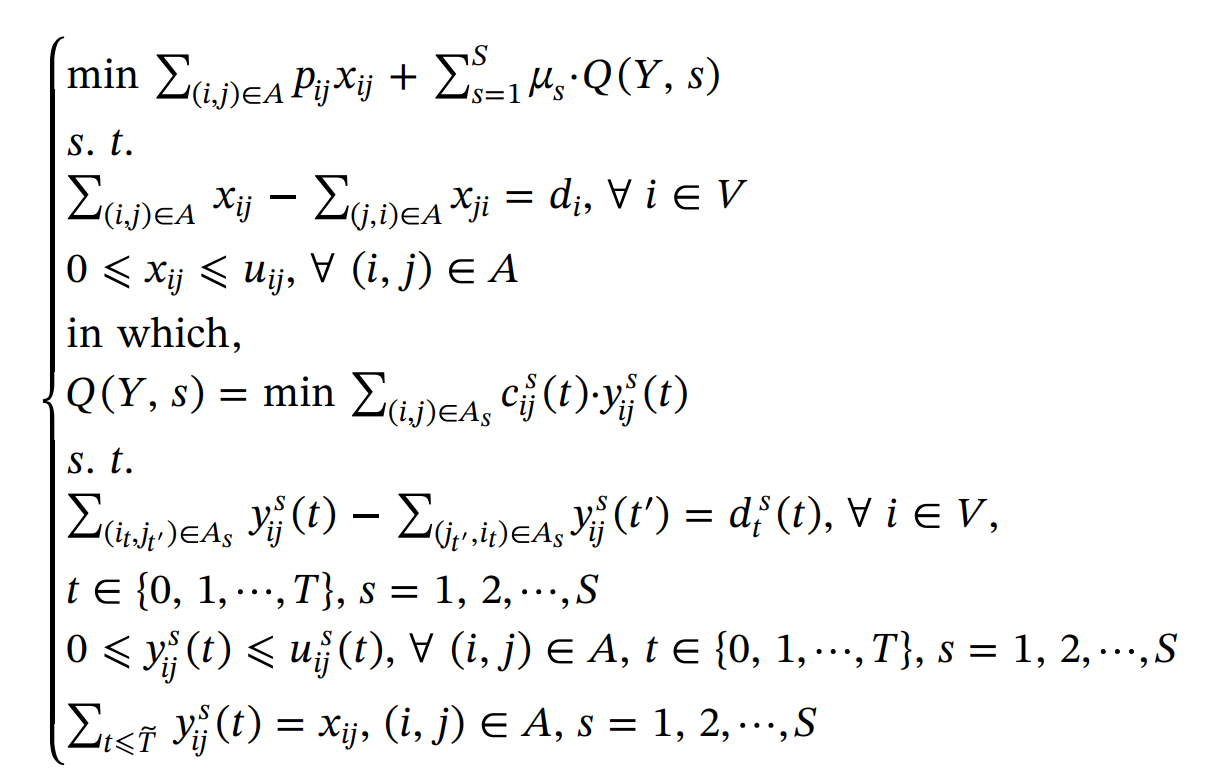
\includegraphics[width=0.5\linewidth]{image.png}  
\end{center}

{Model (time-dependent and random environment) để tìm min của chi phí phạt cho kế hoạch sơ tán ban đầu (priori evacuation) và thời gian di chuyển kì vọng của kế hoạch sơ tán ứng với từng kịch bản. Mục tiêu là tìm kế hoạch sơ tán tối ưu. Vì số kịch bản là có giới hạn nên ta có model tương đương:}

    \begin{center}
      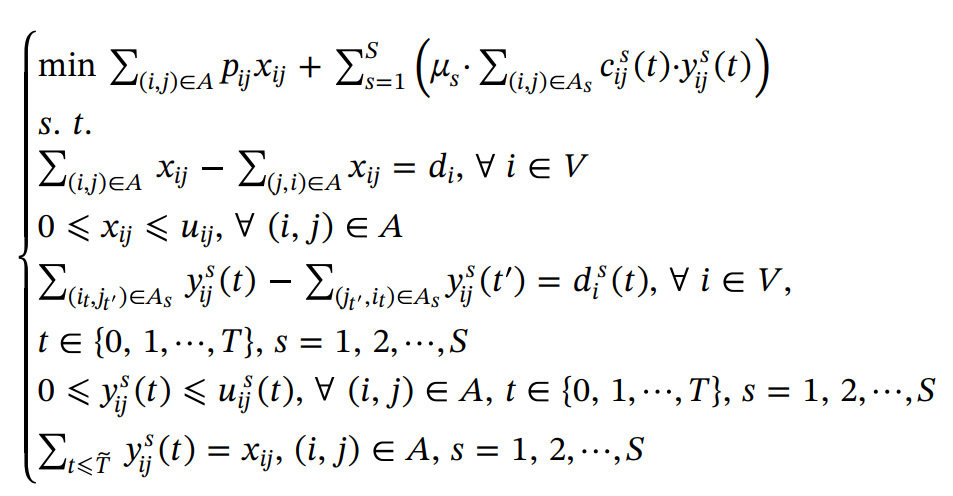
\includegraphics[width=0.5\linewidth]{image1.png}  
    \end{center}

{Trong model này thì travel time và capacity trên mỗi cạnh là các biến ngẫu nhiên phụ thuộc vào kịch bản. Nếu travel time và capacity là hằng số thì model này trở thành một model tất định.}

  {Trong trường hợp thông tin được cập nhật từ original node thì kế hoạch sơ tán ban đầu (priori evacuation) không cần thiết (tương đương với threshold (T) = 0). Khi đó model dựa trên wati-and-see (WAS) cần tìm min của tổng giá trị kì vọng của travel time trong các kịch bản:}  
\begin{center}  
    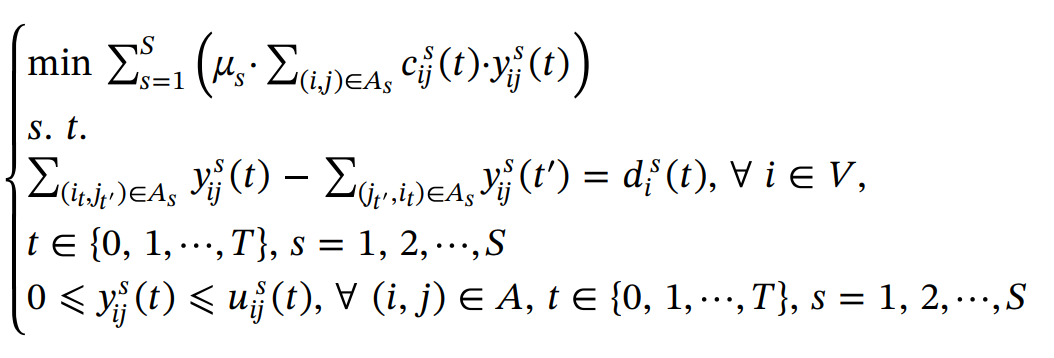
\includegraphics[width=0.5\linewidth]{image2.png}
\end{center}

{Miền khả thi của WAS chứa miền khả thi của model gốc vì vậy nên WAS model là lower bound của model gốc. Vì constraints của các kịch bản khác nhau không có liên hệ với nhau nên có thể chia WAS model thành S sub-problems dựa trên kịch bản. Mỗi kịch bản của model này là một time-dependent min-cost flow problem.}\\

\textbf{Thuật toán giải quyết}

{Coupling constraint là một constraint phức tạp, làm cho model không thể giải được trong thời gian đa thức. Vì vậy nên dùng Lagrangian relaxation approach để relax coupling constraint vào objective function. Phân tích original problem thành 2 sub-problems dễ giải quyết, giá trị tối ưu của 2 sub-problems là lower bound của original model. Original model được chia thành min-cost flow problem tiêu chuẩn và time-dependent min-cost flow problem, có thể được giải bằng thuật toán xác định.}
\begin{enumerate}
    \item[] Dùng nhân tử Lagrange: $\alpha_{ij}^s(t), (i,j) \in A, s = 1, 2,...,S, t\leq \widetilde T$
    \item[] Coupling constraint trở thành: $ \sum_{s=1}^S\sum_{t \leq \widetilde T}\sum_{(i,j)\in A} a_{ij}^s(t)(y_{ij}^s(t)-x_y)$
    \item[] Khi đó original model trở thành:
    \begin{figure}[h]
        \centering
        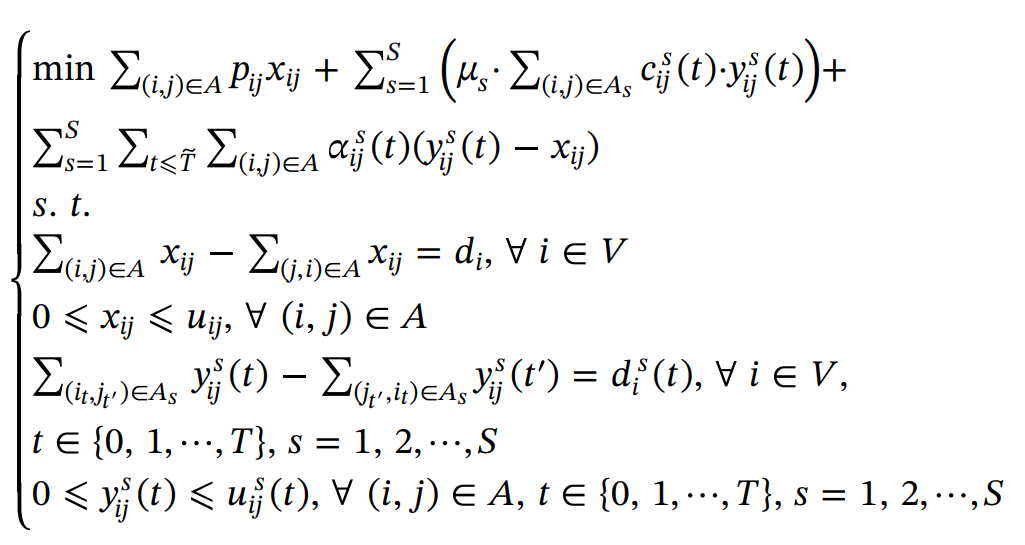
\includegraphics[width=0.5\linewidth]{image3.png}
    \end{figure}
    \newpage
    \item[] Đặt nhân tử chung thì ta sẽ phân tích model thành 2 sub-problems
    \begin{figure}[h]
        \centering
        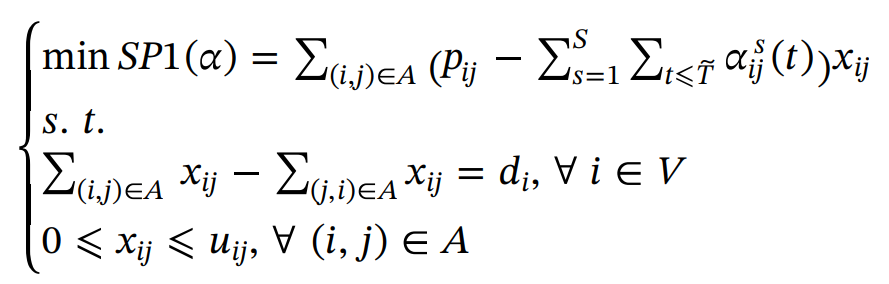
\includegraphics[width=0.5\linewidth]{image4.png}   
    \end{figure}
   
    \item[] Objective function của SubProblem 1:$g_{ij}:= p_{ij} - \sum_{s=1}^S\sum_{t \leq \widetilde T} a_{ij}^s(t)$: chi phí tổng quát
    \item[] SubProblem 1 có thể được giải bằng Successive Shortest Path Algorithm mà chúng tôi sẽ đề cập đến ở phần sau. 
    \begin{figure}[h]
        \centering
        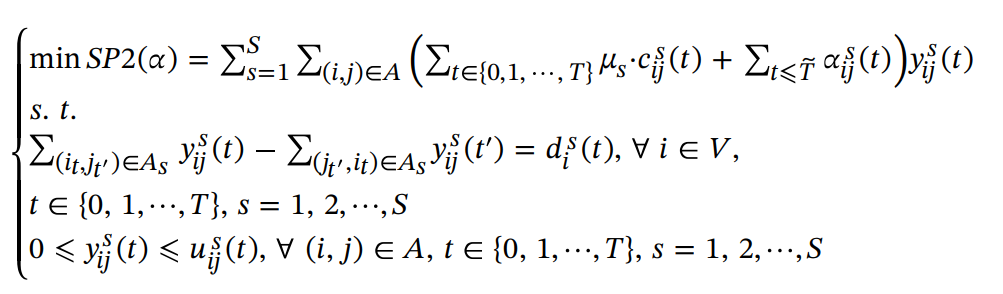
\includegraphics[width=0.6\linewidth]{image5.png} 
    \end{figure}
    \item[] SubProblem 2 có thể được phân tích thành S sub-problems. Mỗi sub-problem là một min-cost flow problem with time-dependent link travel times and capacities.
    \begin{center}
        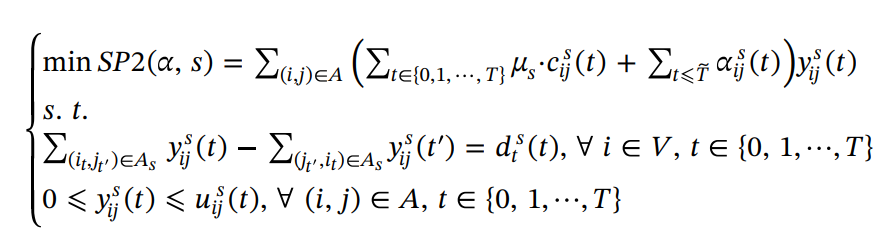
\includegraphics[width=0.5\linewidth]{image6.png}      
    \end{center}
    \item[] Objective fuction của mỗi sub-problem: 
    \begin{center}
        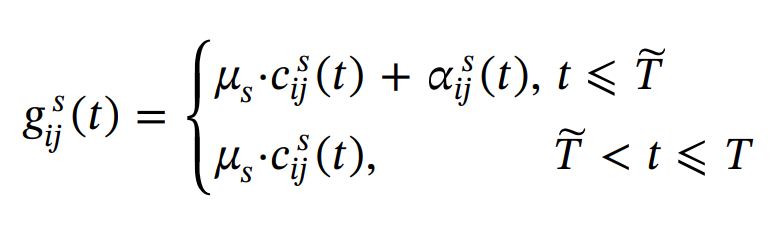
\includegraphics[width=0.35\linewidth]{image7.png}    
    \end{center}
    \item[] Mỗi sub-problem có thể được giải bằng dựa trên Successive Shortest Path Algorithm.
    \item[] Bằng việc giải SubProblem 1 và SubProblem 2, giá trị tối ưu của relaxed model là: $Z_{LR}^*(\alpha) =  Z_{SP1}^*(\alpha)+ Z_{SP2}^*(\alpha)$
    \item[] Giá trị tối ưu của relaxed model là lower bound của giá trị tối ưu của original model. Mục tiêu là tìm ra giá trị tối ưu của relaxed model sao cho nó càng gần giá trị tối ưu của original model càng tốt. Hay giá trị tối ưu của original model là max của relaxed model.
    \[Z_{LD}(\alpha^*) = max_{\alpha \geq 0} Z_{LD}(\alpha)\]
\end{enumerate}


\subsection{Thuật toán Successive Shortest Path}
\subsubsection{Giới thiệu thuật toán}
\subsubsubsection{Đặt vấn đề}
{Trong cuộc sống, đặc biệt là trong công việc quản lí, ta thường xuyên phải bắt gặp các vấn đề về tối ưu số lượng hàng hóa và chi phí vận chuyển. Kịch bản thông thường là cần vận chuyển hàng hóa từ nguồn cung đến vị trí tiêu thụ. Trong quá trình vận chuyển luôn có chi phí phát sinh, vấn đề dành cho những người quản lí là làm sao để điều phối cho số lượng hàng hóa cung cấp đủ nhu cầu và tiết kiệm được nhiều chi phí nhất.}

{Một số ví dụ:}
\begin{enumerate}
    \item[-] {Trong hệ thống giao thông vận tải, logistic: Cần tối ưu hóa lộ trình như thế nào để hàng hóa vận chuyển qua các tuyến đường đáp ứng đủ nhu cầu và chi phí vận chuyển ít nhất.}
    \item[-] {Quản lý lưu lượng internet: tối ưu hóa việc định tuyến dữ liệu thông qua mạng lưới, giảm thiểu độ trễ và tối đa hóa băng thông.}
    \item[-] {Quản lý tài nguyên điện: phân phối điện năng từ nơi tiêu dùng đến nơi tiêu thụ, giúp cân bằng mạng lưới điện, không bị quá tải, giảm thiểu chi phí vận chuyển. }
\end{enumerate}

{Những bài toán hầu như được thực hiện trên những cơ sở dữ liệu lớn, nên chúng ta chỉ có thể giải quyết chúng bằng các phần mềm, lập trình tính toán bằng máy tính. }

{Trong lý thuyết đồ thị của khoa học máy tính, những bài toán tối ưu này được gọi chung là bài toán Min Cost Flow. }
\subsubsubsection{Bài toán Min Cost Flow trong đồ thị }
{Bài toán Min Cost Flow (MCF) là một trong những bài toán quan trọng trong lý thuyết đồ thị và tối ưu hóa. Nó kết hợp hai yếu tố chính là luồng (Flow) và chi phí tối thiểu (Min Cost), và thường được áp dụng trong các vấn đề vận chuyển, lên kế hoạch sản xuất, và quản lý tài nguyên.}

{Mục tiêu bài toán là vận chuyển tài nguyên qua đồ thị (network) sao cho lượng tài nguyên vận chuyển là nhiều nhất và chi phí trong quá trình vận chuyển là ít nhất. }

{Mô hình hóa bài toán trên bằng đồ thị $G=(V,E)$ với:}
\begin{enumerate}
    \item[-] {V là tập hợp các nút (đỉnh) trong đồ thị.}
    \item[-] {E là tập hợp các cạnh, mỗi cạnh (u,v) đại diện cho một liên kết từ nút u đến nút v.}
    \item[-] {$C_{ij}$ là chi phí vận chuyển 1 đơn vị từ đỉnh i đến j}
    \item[-] {$U_{ij}$ là lưu lượng tối đa có thể thông qua trên cạnh ij (capacity) }
    \item[-] {$X_{ij}$ là lưu lượng đi qua cạnh ij } 
\end{enumerate}

{Đồ thị có một nút được chỉ định là nút nguồn s và một nút là nút đích t. Luồng được chuyển từ nút nguồn s đến nút đích t.}

{Mục tiêu:}
\begin{enumerate}
    \item[-] {Luồng trên mỗi cạnh không vượt quá dung lượng của cạnh: $0 \leq f_{u,v} \leq cap_{u,v}$.}
    \item[-] {Luồng vào mỗi nút (trừ nút nguồn và nút đích) bằng luồng ra khỏi nút đó: $\sum_{u}f_{u,v}=\sum_{u}f_{v,u}$.}
    \item[-] {Tối thiểu hóa tổng chi phí của luồng: $\sum_{u,v \in E}f_{u,v}~.~c_{u,v}$ là nhỏ nhất.} 
\end{enumerate}
\subsubsection{Mô tả thuật toán}
\subsubsubsection{Ý tưởng}
{Successive Shortest Path là sự kết hợp giữa 2 bài toán tìm đường đi ngắn nhất và tìm luồng cực đại trong đồ thị. }
\begin{enumerate}
    \item[1.] {Tìm đường đi ngắn nhất:}
    \begin{enumerate}
        \item[-] {Bắt đầu với việc tìm đường đi ngắn nhất từ nút nguồn đến các nút khác trong đồ thị. }
        \item[-] {Đường đi này được tìm đựa trên trọng số và chi phí của các cạnh.} 
    \end{enumerate}
    \item[2.] {Cải thiện luồng}
    \begin{enumerate}
        \item[-] {Áp dụng thông tin từ đường đi ngắn nhất để cải thiện luồng.}
        \item[-] {Cải thiện luồng bằng cách thay đổi luồng trên các cạnh theo đường đi tối ưu để giảm chi phí hoặc tối ưu lưu lượng.} 
    \end{enumerate}
    \item[3.] {Lặp lại quá trình}
    \begin{enumerate}
        \item[-] {Tiếp tục lặp lại quá trình tìm đường đi ngắn nhất và cải thiện luồng cho đến khi không thể cải thiện được nữa hoặc khi đạt đến điều kiện dừng.}
    \end{enumerate}
\end{enumerate}

\begin{figure}[h]
    \centering
    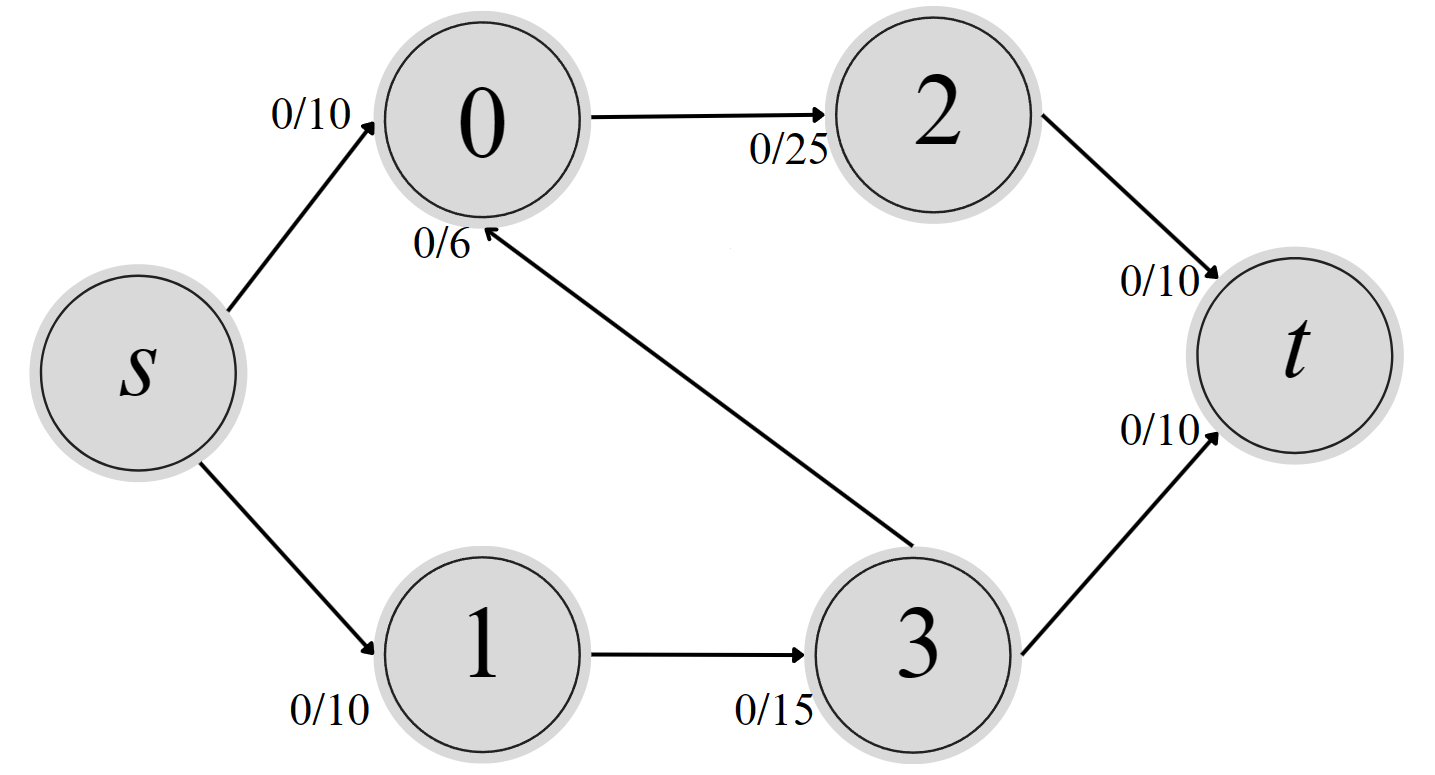
\includegraphics[width=0.5\linewidth]{graph.png}
    \caption{Initial Graph}
    \label{fig:enter-label}
\end{figure}

{Để hiện thực giải thuật SSP, nhóm quyết định sử dụng giải thuật luồng cực đại Fulkerson và giải thuật đường đi ngắn nhất Dijkstra.}
\subsubsubsection{Giải thuật luồng cực đại Fulkerson}
{Một số khái niệm cơ bản:}
\begin{enumerate}
    \item[-] {Initial Graph (đồ thị đơn giản ban đâu): Thuật toán FKS sử dụng các đồ thị gồm 1 nguồn, và 1 đích G(V,E) với:}
    \begin{enumerate}
        \item[+] {V là tập hợp các nút (đỉnh) trong đồ thị.}
        \item[+] {E là tập hợp các cạnh, mỗi cạnh (u,v) đại diện cho một liên kết từ nút u đến nút v.}
        \item[+] {$C_{ij}$ là chi phí vận chuyển 1 đơn vị từ đỉnh i đến j}
        \item[+] {$U_{ij}$ là lưu lượng tối đa có thể thông qua trên cạnh ij (capacity) }
        \item[+] {$X_{ij}$ là lưu lượng đi qua cạnh ij } 
    \end{enumerate}
    \item[-] {Forward Edge: các cạnh có hướng trong đồ thị ban đầu được tạo}
    \item[-] {Backward Edge (Arc): là cạnh ngược chiều tương ứng với từng Forward Edge trong đồ thị ban đầu. Backward Edge có giá trị flow ban đầu là 0, giá trị capacity ban đầu cũng là 0. }
    \item[-] {Residual graph (đồ thị thặng dư): Là đồ thị bao gồm đồ thị bao gồm các Forward Edge và Backward Edge, có thể hiểu là biểu đồ hoàn trả flow. Trong biểu đồ này ta có thể hoàn trả flow từ các cạnh khác nhau và chuyển hướng của chúng đến vị trí hợp lí hơn để đạt được maxflow. Biểu đồ Residual giống hệt đồ thị ban đầu, chỉ khác là ta thêm các Backward Edge (arc) vào đồ thị ban đầu (để có thể hoàn trả flow giữa các luồng). Các cạnh giả này có hệ số flow, capacity ban đầu là 0/0. Mọi thao tác của thuật toán Fulkerson đề thực hiện trên đồ thị Residual graph.} 
    \begin{figure}[h]
        \centering
        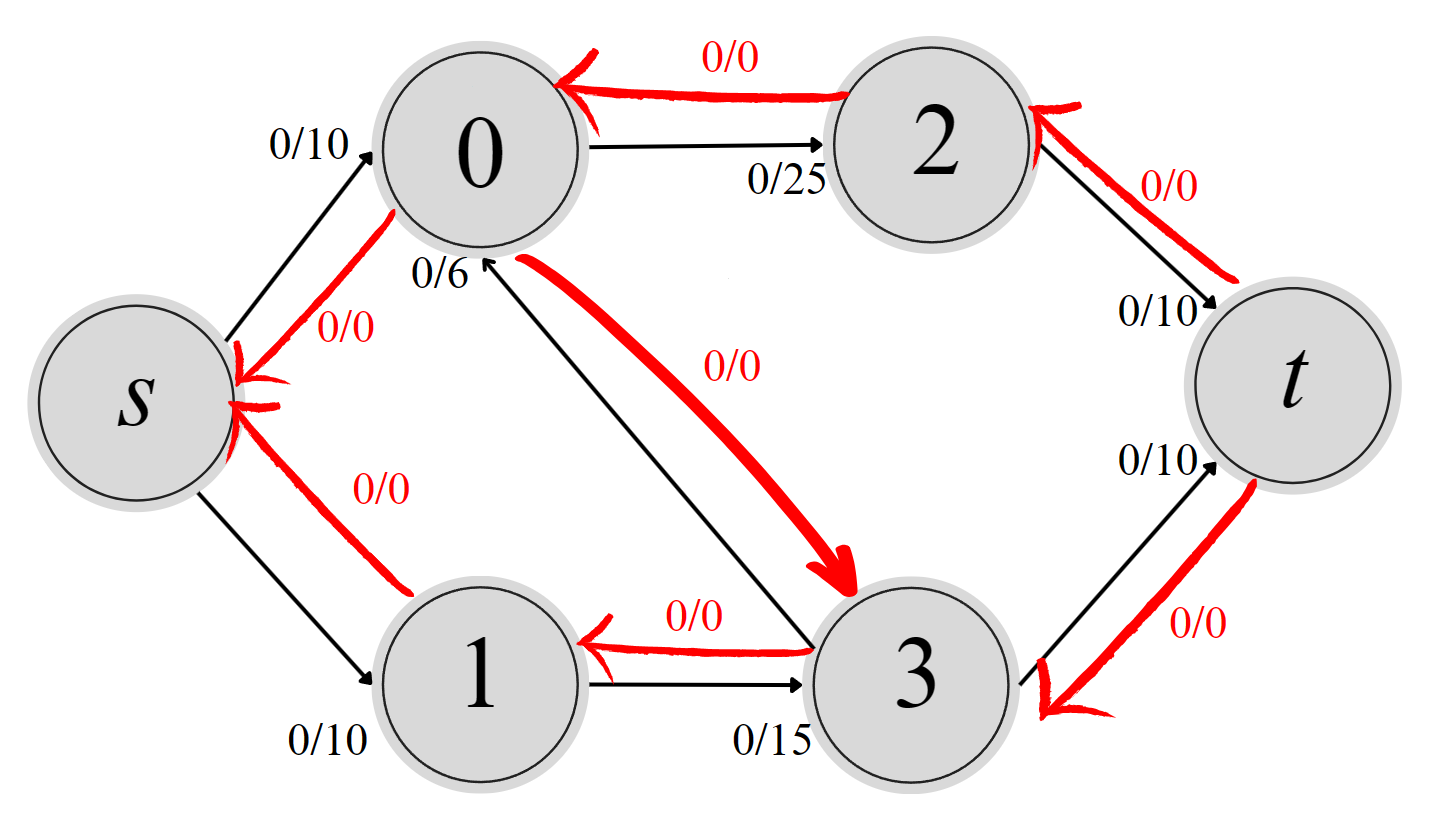
\includegraphics[width=0.5\linewidth]{graph1.png}
        \caption{Residual graph}
        \label{fig:enter-label}
    \end{figure} 
    \item[-] {Augmenting path (luồng tăng cường): đường đi mà flow trên mỗi cạnh chưa tối đa  ${flow}_{i} < {capacity}_i$. } 
    \item[-] {Bottleneck value: Duyệt theo augmenting path, tìm giá trị nhỏ nhất trong số $capacity_i  - flow_i$ (remaing capacity). Có thể hiểu Bottleneck value là giá trị flow lớn nhất có thể tăng thêm thông qua Augmenting path (tức là tăng sao cho flow trên	 mỗi cạnh đường đi vẫn thỏa $flow_i \leq capacity_i$).} 
\end{enumerate}
{Thuật toán Ford Fulkerson: là hành động lặp đi lặp lại việc tìm augmenting path đến khi không tìm thấy augmenting path nữa hoặc luồng tại sink đã bằng tại source. Có rất nhiều đường đi để flow đạt cực đại, thuật toán Ford Fulkerson chỉ tìm lượng cực đại chứ không quan tâm đến đường đi. Thuật toán thực hiện các bước sau: }
\begin{enumerate}
    \item[1.] {Khởi tạo biến maxflow = 0}
	\item[2.] {Tìm augmenting path trên residual graph: tìm ngẫu nhiên, có thể tuân theo DFS, nếu không tìm được argumeting path hoặc flow tại sink = flow tại source thì dừng (augmenting path có thể chứa undo edge, khi đó ta có thể hiểu flow qua undo edge hiện tại là lượng trả ngược lại cho một augmenting path trước đó để chừa khoảng trống cho lượng flow khác đi qua). }
	\item[3.] {Tìm Bottleneck (G) value trên augmenting path. Cập nhập maxflow += G}
	\item[4.] {Cập nhập lại residual graph.}
 \begin{center}
\begin{matrix}
 \text{forward edge in argumenting } $path_i~+= G$ \\
 \text{backward edge in argumenting } $path_i~-= G$
\end{matrix}
 \end{center}
	\item[5.] {Lặp lại bước 1}
\end{enumerate}
\(\Rightarrow\) {Giá trị biến maxflow là luồng cực đại có thể đi qua đồ thị.}\\

{Độ phức tạp:}

{Trong bài toán chúng ta đang xét, tất cả các khả năng thông qua của các cạnh đều là số nguyên. Do đó, mỗi bước tăng luồng đều làm tăng giá trị của luồng lên ít nhất 1 đơn vị. Khi sử dụng thuật toán BFS hoặc DFS để tìm đường tăng luồng, độ phức tạp sẽ vào cỡ $O(E)$. Dó đó, độ phức tạp của phương pháp Ford Fullkerson sẽ là $O(Ef)$, với $f$ là giá trị của luồng cực đại trên mạng. Đây không phải là một độ phức tạp với thời gian đa thức trên kích thước đồ thị.}
\subsubsubsection{Giải thuật tìm đường đi ngắn nhất Dijkstra}
{Thuật toán Dijkstra được sử dụng để tìm đường đi ngắn nhất từ một đỉnh nguồn đến tất cả các đỉnh còn lại trong đồ thị. Đây là thuật toán rất phổ biến và hiệu quả để giải quyết vấn đề tìm đường đi ngắn nhất trong các hệ thống mạng lưới, định tuyến trong mạng máy tính, hoặc trong các bài toán liên quan đến tối ưu hóa đường đi. Một điều kiện để sử dụng được Dijkstra là đồ thị không có chu trình âm. }

{Ý tưởng cơ bản của thuật toán:}
\begin{enumerate}
    \item[1.] {Khởi tạo: Đặt khoảng cách từ đỉnh nguồn đến chính nó là 0 và đặt khoảng cách tất cả các đỉnh khác là vô cùng lớn (hoặc một giá trị lớn đủ lớn).}
    \item[2.] {Lặp: Lặp qua tất cả các đỉnh:} 
    \begin{enumerate}
        \item[\bullet] {Chọn đỉnh có khoảng cách nhỏ nhất từ nguồn mà chưa được xử lý.}
        \item[\bullet] {Cập nhật khoảng cách của tất cả các đỉnh kề với đỉnh được chọn, nếu khoảng cách mới tốt hơn khoảng cách hiện tại.}
    \end{enumerate}
    \item[3.] {Đánh dấu: Đánh dấu đỉnh đã được xử lý.} 
    \item[4.] {Lặp lại bước 2 và 3 cho đến khi tất cả các đỉnh đều đã được xử lý.} 
\end{enumerate}

{Thuật toán này sử dụng một cấu trúc dữ liệu như hàng đợi ưu tiên (priority queue) để lựa chọn đỉnh tiếp theo cần xử lý, giúp tối ưu hóa thời gian xử lý. Nó chắc chắn sẽ tìm ra đường đi ngắn nhất từ đỉnh nguồn đến tất cả các đỉnh còn lại trong đồ thị.}

{Một điều thoáng qua có thể thấy rằng, việc lựa chọn giải thuật Dijkstra để kết hợp với thuật toán Fulkerson gây mâu thuẫn. Vì trong thuật toán Fulkerson có sử dụng đồ thị thặng dư (residual graph) mang trọng số âm. Tuy nhiên vấn đề này không hề gây ảnh hướng đến giải thuật Successive Shortest Path, chúng ta sẽ bàn kĩ hơn về vấn đề này ở phần sau}

{Độ phức tạp thông thường của thuật toán trên sẽ là $O(V^2)$. Nếu ta sử dụng một hàng đợi ưu tiên (priority queue) và sử dụng danh sách kề thì độ phức tạp của thuật toán sẽ bị giảm xuống còn $O((V+E)∗logV)$.}

{Nguyên nhân là, với danh sách kề, thời gian để duyệt các cạnh và các đỉnh sẽ là $O(E+V)$ thay vì $O(V^2)$ như ma trận kề. Với piority queue, việc tìm đỉnh gần nhất ở sẽ chỉ còn $O(1)$ thay vì $O(V)$. Vì thế ta cần nhập khoảng cách tới các đỉnh xung quanh vào binary heap bằng cách bỏ các đỉnh đó ra khỏi heap rồi thêm lại, cái này mất $O(logV)$.}

{Vậy cuối cùng độ phức tạp sẽ là $O((V+E)∗logV)$.}
\subsubsubsection{Giải thuật Successive Shortest Path}
{Thuật toán successive Shortest Path là sự kết hợp thuật toán tìm đường đi ngắn nhất và thuật toán luồng cực đại. Thuật toán này sẽ lặp lại việc tìm đường đi với chi phí thấp nhất trong đồ thị thặng dư (residual graph) rồi thực hiện tăng cường luồng trên đường đi này. }

{Để có thể thực hiện thuật toán tìm đường đi với chi phí thấp nhất, ta thêm mỗi cạnh trong residual graph một thuộc tính cost, nếu forward edge có $cost = A$ thì backward edge có $cost = -A$}

{Các bước thực hiện: }
\begin{enumerate}
    \item[1.] {Khởi tạo biến $maxflow = 0,~mincost = 0$}
    \item[2.] {Tìm augmenting path trên residual graph: }
    \begin{enumerate}
        \item[\bullet] {Tìm bằng giải thuật Dijikstra sao cho cost trên đường đi là nhỏ nhất.}
        \item[\bullet] {Nếu không tìm được argumeting path hoặc flow tại $sink = flow$ tại source ($maxflow = v$) thì dừng (augmenting path có thể chứa undo edge, khi đó ta có thể hiểu flow qua undo edge hiện tại là lượng trả ngược lại cho một augmenting path trước đó để chừa khoảng trống cho lượng flow khác đi qua). }
    \end{enumerate}
    \item[3.] {	Tìm Bottleneck (G) value trên augmenting path. Cập nhập $maxflow~+= G$. Trong quá trình tìm bottleneck thì cập nhập $mincost~+= cost of edge in augmenting path_i$} 
    \item[4.] {Cập nhập lại residual graph. } 
    \begin{center}
        \begin{matrix}
            \text{forward edge in argumenting }$path_i~+= G$\\
            \text{backward edge in argumenting }$path〗_i~-= G$
        \end{matrix}
    \end{center}
    \item[5.] {Lặp lại bước 1} 
\end{enumerate}
\(\Rightarrow\) {Giá trị biến maxflow và mincost tìm được}\\
{Mã giả:}
\begin{mdframed}
    [hidealllines=true,backgroundcolor=gray!10]

\begin{lstlisting}
Tranform network G by adding source and sink
Initial flow x is zero
while (GX contains a path P from s to t) do
    Find any shortest path P from s to t
    Augment current flow x along P
    update GX
    
\end{lstlisting}
\end{mdframed}
\textbf{Giải thích việc lựa chọn thuật toán Dijkstra: }

{Để giải quyết bài toán SSP ta có thể sử dụng nhiều thuật toán tìm đường đi ngắn nhất khác như: Bellman-Ford, Floyd-Warshall,… Nhưng nhóm quyết định chọn thuật toán Dijkstra. Nhưng liệu có hợp lí khi Dijkstra được sử dụng trên đồ thị trọng số âm (residual graph) hay không? Chúng ta có thể chứng minh trong quá trình cập nhập residual graph không thể tạp ra chu trình âm đối với cost.}

{Gọi residual graph đang xét là $G$. Tại thời điểm ban đầu, mọi trọng số flow trên các forward edge và backward edge đều lớn hơn hoặc bằng 0, nên cách cạnh ngược không được xét đến, vậy không thể xảy ra chu trình âm. Giả sử rằng sau một vài thao tác tăng cường luồng, chúng ta có flow $e$ và lúc này $G_e$ vẫn chưa có chu trình âm. Nếu $e$ là giá trị luồng cực đại tối ưu thì kết thúc bài toán. Ngược lại, chúng ta tiếp tục tăng cường luồng, gọi luồng tăng cường với chi phí thấp nhất của $G_e$ là $P$. Giả sử rằng, sau thao tác tăng cường luồng $P$ thì chu trình âm $W$ xuất hiện. Bởi vì trước đó không xuất hiện chu trình âm, nên chắc chắn trong $P$ tồn tại một cạnh $(i,j)$ (gọi là $x$) nào đó mà cạnh ngược $(j,i)$ (gọi là $y$) của nó làm khép kín chu trình âm $W$.}
\begin{center}
    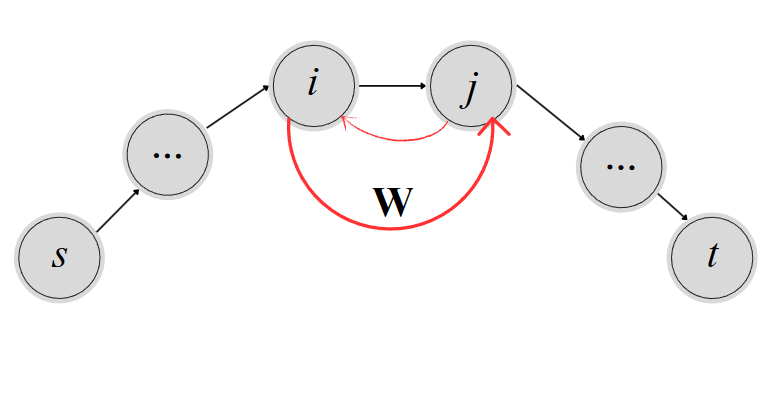
\includegraphics[width=0.5\linewidth]{huy1.png}   
\end{center}

{Lúc này tồn tại 2 đường đi từ $i$ đến $j$, một đường đi là cạnh $x$, đường đi còn lại gọi là $T$. Bởi vì trọng số cost trên $x$ và $y$ là đối nhau nên chu trình âm $W$ chúng ta đang nhắc đến không được tạo bởi $x$ và $y$. Vậy phải có đường đi khác từ $i$ đến $j$ để kết hợp với $y$ tạo ra chu trình âm $W$. Lúc này chu trình âm $W$ là $(T,y)$. }

{Kí hiệu $f(a)$ là tổng trọng số cost trên đường đi $a$. Bởi vì $(T,y)$ là chu trình âm nên $f(T) + f(y) < 0$. Ta xét đến 2 trường hợp $f(T) > 0$ và $f(T) < 0$ khi đó: }
\[
\left\{\begin{matrix}
f(T) + f(y) < 0\\
 f(y) < 0
\end{matrix}\right.
\Leftrightarrow f(T) <  \left|f(y) \right|
\]

{Mà ta lại có $f(y) = -f(x)$ với $f(x) > 0$ nên ta suy ra $f(T) < f(x)$. Lúc này tồn tại một đường đi theo thứ tự từ đỉnh nguồn $s$ đến $i$, từ $i$ đến $j$ thông qua $T$ (thay vì thông qua $x$), từ $j$ đến đỉnh đích $t$. Chắc chắn đường đi này có chi phí thấp hơn $P$. Điều này tạo ra mâu thuẫn với giả thuyết ban đầu $P$ là đường đi có chi phí thấp nhất. }

{Vậy việc cập nhập residual không thể tạo ra chu trình âm nên việc chọn thuật toán Dijkstra là hoàn toàn khả thi. Việc chọn Dijkstra mang lại hiệu suất tốt hơn cho thuật toán Successive Shortest Path thay vì chọn các thuật toán đường đi ngắn nhất khác. }
\subsubsection{Thử nghiệm thuật toán}
\subsubsubsection{Sinh đồ thị ngẫu nhiên}
{Sau khi trình bày về giải thuật Successive Shortest Path, chúng ta đến với các thao tác để tạo nên đồ thị để kiểm tra giải thuật. Để kiểm tra hiệu quả hơn chúng tôi sẽ tìm cách sinh ra các đồ thị có hướng ngẫu nhiên thỏa mãn 1 nguồn, 1 đích. Chúng tôi sẽ đề cập đến 2 đồ thị gồm: }
\begin{enumerate}
    \item[-] {Đồ thị có hướng thuông thường gồm 1 nguồn 1 đích (gọi tắt là NormalGraph) }
    \item[-] {Đồ thị có hướng theo dạng lưới (grid network) gồm 1 nguồn 1 đích (gọi tắc là NetworkGraph), đồ thị này đã được đề cập trong phần 5.1 bài báo của Li-Wang. } 
\end{enumerate}
\textbf{Cách sinh ngẫu nhiên Normal Graph}

{Mục tiêu: Sinh ra đồ thị với số node và link cho trước.  Giả sử số lượng node là $n$ và số lượng link là $m$}

{Ý tưởng: Chúng ta sẽ tạo ra một đồ thị đầy đủ cho số lượng node đã biết. Vậy đồ thị tạo ra có $n$ nodes và $n(n-1)$ links. Ta sẽ thực hiện xóa ngẫu nhiên các cạnh trên đồ thị đến khi đủ $m$ cạnh. Lưu ý rằng thao tác xóa này phải đảm bảo rằng đồ thị thu được gồm 1 nguồn và 1 đích. } 

{Các bước hiện thực:} 
\begin{enumerate}
    \item[] {\textit{Step 1:} Tạo đồ thị đầu đủ ban đầu: }
    \item[] {Sử dụng random ma trận trong python để tạo nên ma trận trọng số có cỡ nxn. Ta sẽ random 2 ma trận cùng lúc là ma trận capacity và cost tương ứng, mọi thao tác trên 2 ma trận này đều đồng nhất với nhau. }
    \item[] {Quy ước rằng giá trị $arr[i][j]$ là trọng số của đồ thị (capacity và cost) trên cạnh từ $I$ đến $j$. Đỉnh nguồn của đồ thị luôn là 0 còn đỉnh đích là $n-1$ (n là số nodes của đồ thị). Nếu $arr[i][j] = 0$ thì không có đường đi giữa 2 đỉnh $I$ và $j$. } 
    \begin{figure}[h]
        \centering
        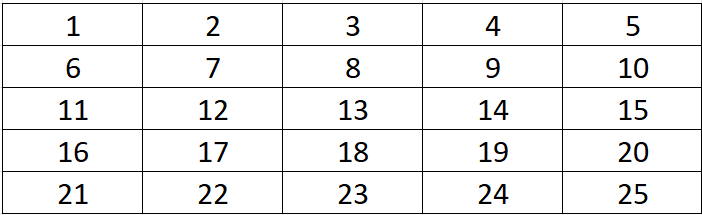
\includegraphics[scale=0.8]{table_2.png}
        \caption{Ví dụ minh họa random man trận trọng số của đồ thị có 5 nodes}
        \label{fig:enter-label}
    \end{figure}
    \item[] {\textit{Step 2:} Đưa đồ thị về một nguồn, một đích. } 
    \item[] {Thực hiện xóa các cạnh vòng ở mỗi đỉnh, xóa cách cạnh đi vào đỉnh nguồn và xóa các cạnh đi ra khỏi đỉnh đích. } 
    \begin{figure}[h]
        \centering
        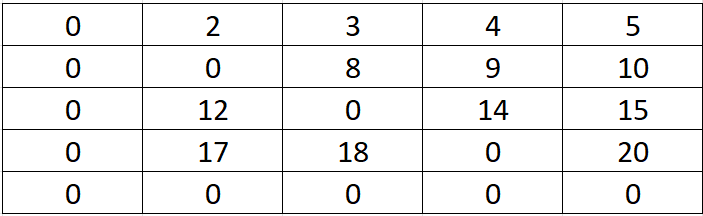
\includegraphics[scale=0.8]{table_3.png}
        \caption{Ví dụ cho ma trận trọng số của đồ thị có 5 nodes sau thao tác này}
        \label{fig:enter-label}
    \end{figure}
    \item[] {Ta cần tính toán số lượng link còn lại sau thao tác xóa ban đầu này. Thao tác này nhằm kiểm soát được khi nào số lượng cạnh của đồ thị bằng số lượng cạnh yêu cầu.}
    \item[] {$Links~now = NODES \ast NODES - 3 \ast NODES + 3$} 
    \item[] {\textit{Step 3:} Xóa dần các cạnh đến khi đủ $m$ cạnh cho trước} 
    \item[] {Muốn xóa các cạnh để thu được đồ thị 1 nguồn, 1 đích, ta cần quan tâm đến các bán bậc ra và bán bật vào của từng đỉnh. Ta thực hiện tính toán mảng các giá trị bán bậc ra và vào của các đỉnh trên đồ thị lúc này. }
    \item[] {Tiếp theo ta cần chọn các cạnh còn lại trong đồ thị rồi xóa đi. Điều này có nghĩa rằng ta sẽ chọn 1 giá trị bất kì trong ma trận trọng số đồ thị rồi gán cho giá trị bằng 0. Tuy nhiên việc lựa chọn này có vài điều kiện kèm theo. } 
    \item[] {Giả sử ô ta muốn chọn trên ma trận trọng số của đồ thị nằm ở hàng $r$ và cột $c$, khi đó: }
    \begin{enumerate}
        \item[\bullet] {$r$ thuộc khoảng $0 \leq r \leq n-2$. Vì hàng tại vị trí $n-1$ đã bằng 0 trước đó}
        \item[\bullet] {$c$ thuộc khoảng $1 \leq c \leq n-1$. Vì cột tại vị trí 0 đã bằng 0 trước đó.} 
    \end{enumerate}
    \item[] {Điều kiện để 1 cạnh bị xóa là: khi cạnh đó mất đi bán bậc ra và bán bậc vào ở 2 đỉnh bên cạnh không bằng 0. Điều này đồng nghĩa với việc thao tác xóa không tạo thêm bất kì đỉnh nguồn hoặc đỉnh đích nào. }
    \item[] {Hơn thế, chúng ta muốn random đồ thị có nhiều cạnh đi ra từ đỉnh nguồn và có nhiều cạnh đi vào đỉnh đích. Điều này nhằm giúp cho việc tính toán có ý nghĩa và hợp lý hơn mỗi khi chúng ta random đồ thị. Vì vậy cần tạo thêm mảng xác suất để lựa chọn các cạnh. Chúng ta quyết định để xác suất chọn và xóa 1 cạnh đi ra từ đỉnh nguồn cũng như đi vào đỉnh đích là $a$. Xác suất để lựa chọn các cạnh còn lại là $3a$. Vậy xác suất chọn và xóa 1 cạnh liên quan đến đỉnh nguồn và đích bằng $1/3$ xác suất chọn các cạnh còn lại. } 
    \item[] {Tiếp theo ta thực hiện việc random cạnh và xóa cạnh đó ra khỏi đồ thì đến khi số lượng cạnh bằng $m$ (links) cho trước. } 
    \begin{figure}[h]
        \centering
        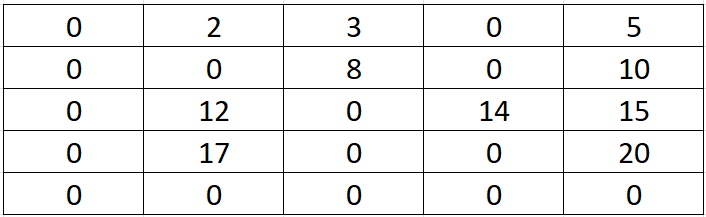
\includegraphics[scale=0.8]{table_4.png}
        \caption{Ví dụ cho ma trận trọng số của đồ thị có 5 nodes sau thao tác này}
        \label{fig:enter-label}
    \end{figure}
    \item[] {\textit{Step 4:} Tạo DataFrame lưu thông tin các cạnh để tiện cho việc sử dụng } 
    \item[] {Kết luận: Việc random đồ thị như trên khá mang tính tổng quát, tốt hơn việc định hình sẵn đồ thị rồi random các trọng số trên đó. Đồ thị được sinh ra với các cạnh ngẫu nhiên nhưng vẫn đảm bảo có đúng 1 nguôn và 1 đích.} 
    \begin{figure}[h]
  \centering
  \subfigure{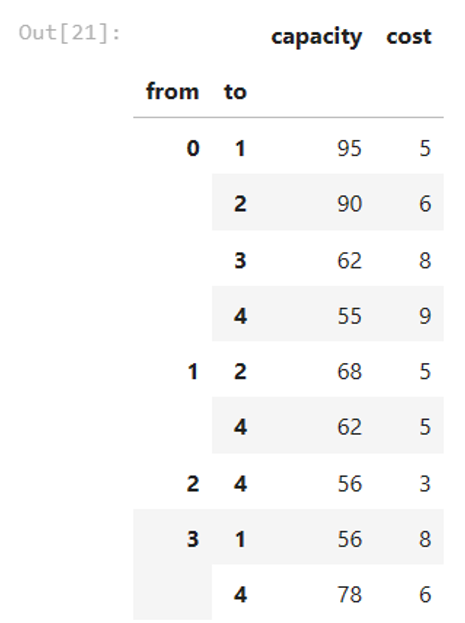
\includegraphics[width=0.33\linewidth]{example.png}}
  \hfill
  \subfigure{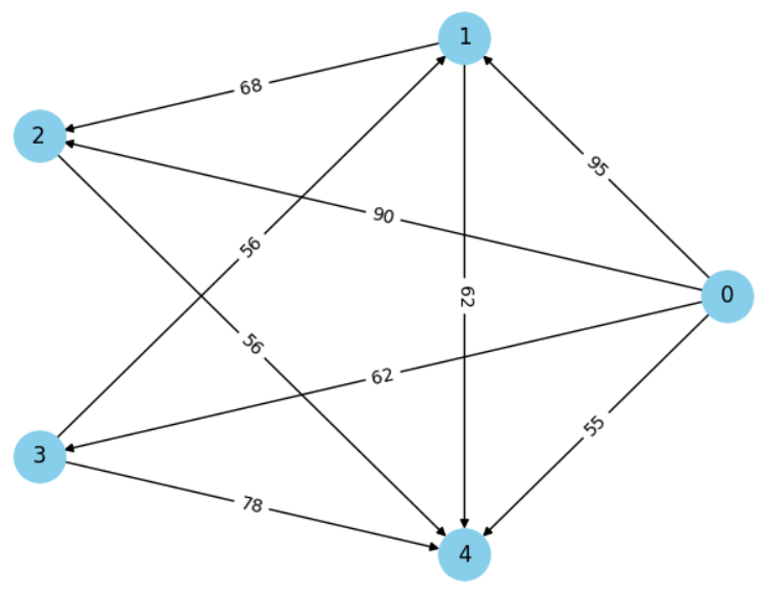
\includegraphics[width=0.6\linewidth]{example1.png}}
  \caption{Ví dụ minh họa cho DataFrame thu được: }
\end{figure}
\end{enumerate}
\newpage
\textbf{Sinh ngẫu nhiên đồ thị Network Graph}

{Mục tiêu: sinh ra đồ thị dạng lưới giống trong bài báo của LiWang}
\begin{figure}[h]
    \centering
    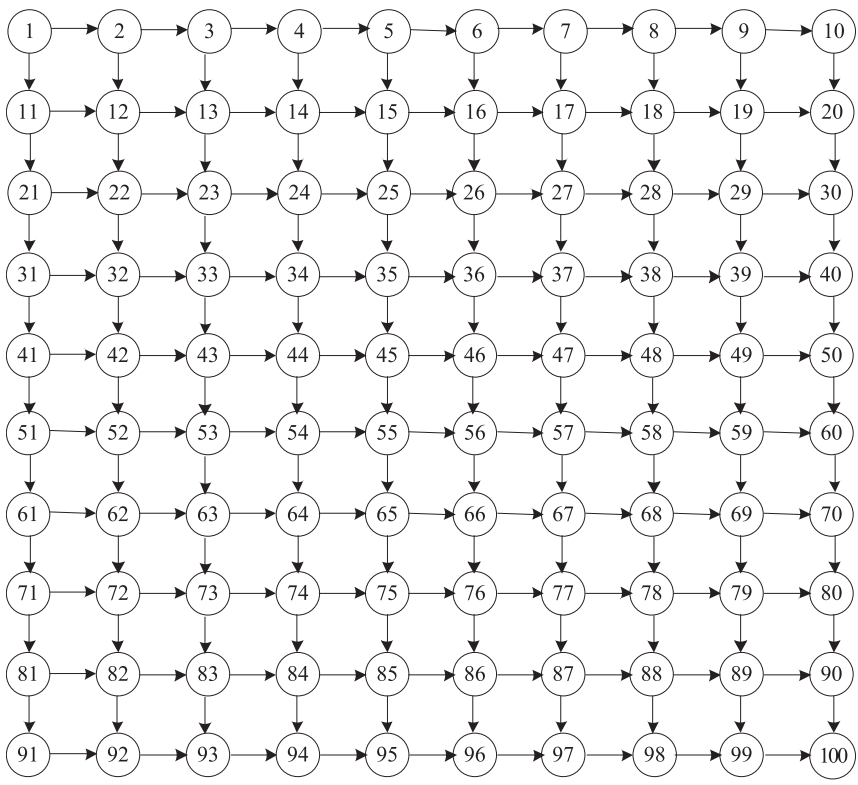
\includegraphics[scale=0.8]{grid.png}
    \caption{A Grid Network.}
    \label{fig:enter-label}
\end{figure}
\newpage
{Nhận xét: đồ thị dạng lưới như ma trận vuông có size 10x10 nên ta sẽ sinh đồ thị dạng lưới với size cho trước. Đồ thị có các liên kết tuân theo quy luật: Node thứ i sẽ nối với node thứ $i+1$ và node thứ $i+size$. Trừ một số trường hợp: }

{Ý tưởng: Sử dụng ma trận vuông với size cho trước. Chỉ random trọng số tại các vị trí có liên kết, các vị trí còn lại đều mang giá trị 0.}

{Các bước hiện thực: }
\begin{enumerate}
    \item[] {\textit{Step 1:} Tạo ma trận trọng số cost và capacity tương ướng, khởi tạo ma trận ban đầu tất cả các giá trị đều bằng 0. Mọi thao tác trên 2 ma trận này đều đồng nhất với nhau.}
    \item[] {\textit{Step 2:} Duyệt qua ma trận, kiểm tra điều kiện nếu là vị trí có cạnh thì random trọng số tại vị trí đó. (Ta không cần xét điều kiện cho các node ở biên dưới, vì khi này i+size đã vượt quá chỉ số của ma trận)}
    \item[] {\textit{Step 3:} Lọc dữ liệu các cạnh đã thu được vào DataFrame để dễ sử dụng và quan sát. } 
\begin{enumerate}
    \item[\bullet] {Node nằm ở biên phải, tức là khi i chia hết cho size. }
    \item[\bullet] {Node nằm ở biên dưới.}  
\end{enumerate}
\end{enumerate}
\begin{tcolorbox}[colback=blue!5!white,colframe=blue!75!black, title= \text{Ví dụ minh họa cho ma trận trọng số của đồ thị có $size = 3 \times ơ3$} ]
\begin{verbatim}
[ 0. 76.  0. 77.  0.  0.  0.  0.  0. ]
[ 0.  0. 79.  0. 90.  0.  0.  0.  0. ]
[ 0.  0.  0.  0.  0. 99.  0.  0.  0. ]
[ 0.  0.  0.  0. 88.  0. 51.  0.  0. ]
[ 0.  0.  0.  0.  0. 86.  0. 77.  0. ]
[ 0.  0.  0.  0.  0.  0.  0.  0. 98. ]
[ 0.  0.  0.  0.  0.  0.  0. 73.  0. ]
[ 0.  0.  0.  0.  0.  0.  0.  0. 99. ]
[ 0.  0.  0.  0.  0.  0.  0.  0.  0. ]
\end{verbatim}
\end{tcolorbox}
\begin{figure}[h]
    \centering
    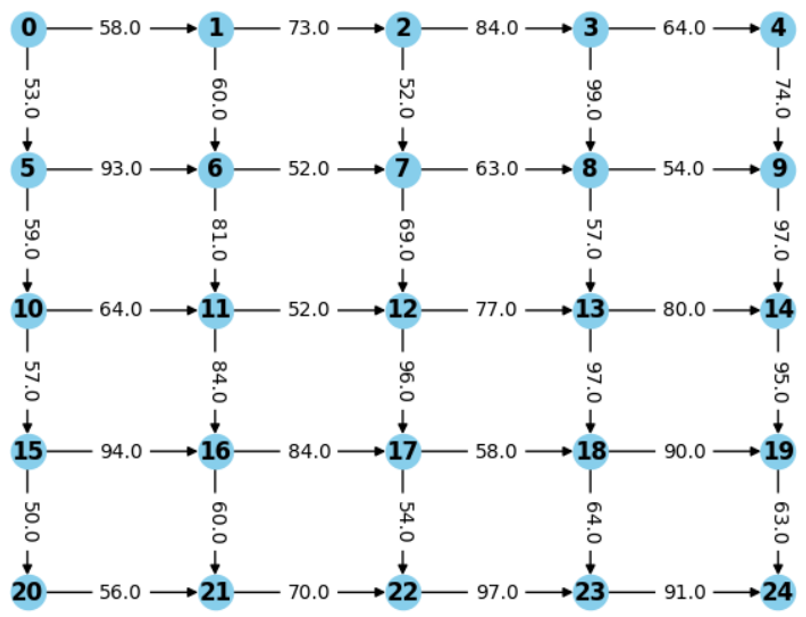
\includegraphics[scale=0.9]{grid1.png}
    \caption{Ví dụ đồ thị thu được }
    \label{fig:enter-label}
\end{figure}

\subsubsubsection{Một số kết quả}
{\textit{Chú ý}: Đối với mỗi đồ thị luôn có source là node bé nhất (node 0) và sink là node lớn nhất (node $n-1$)}
\begin{figure}[h]
  \centering
  \subfigure{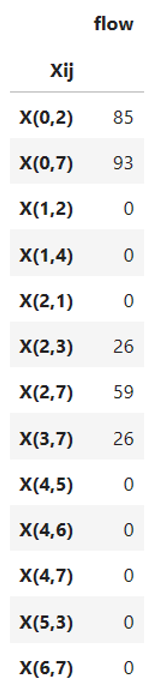
\includegraphics[width=0.15\linewidth]{flow.png}}
  \hfill
  \subfigure{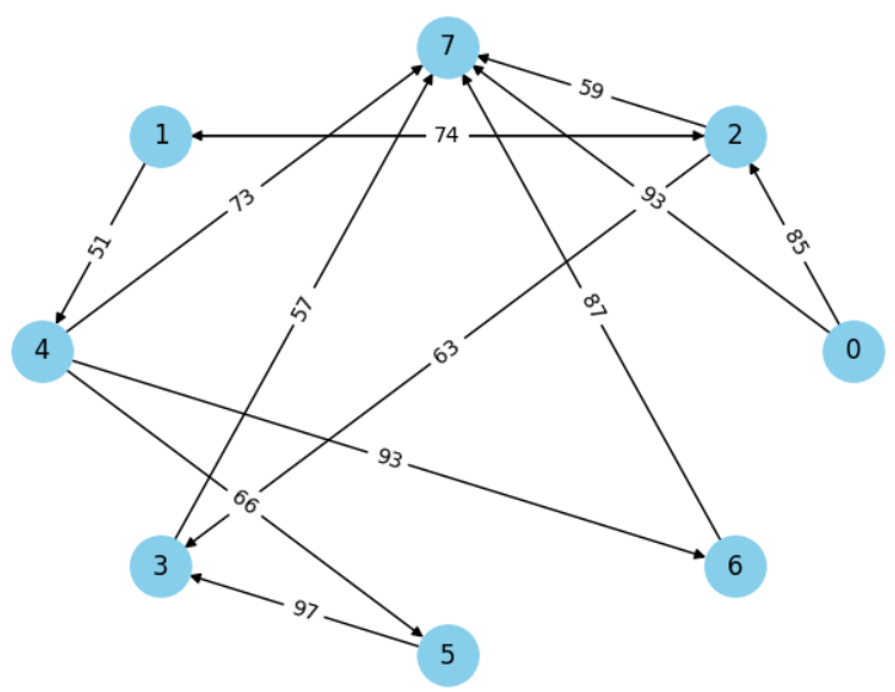
\includegraphics[width=0.8\linewidth]{normal_graph.png}}
  \caption{Đối với Normal Graph}
\end{figure}

\begin{figure}[h]
  \centering
  \subfigure{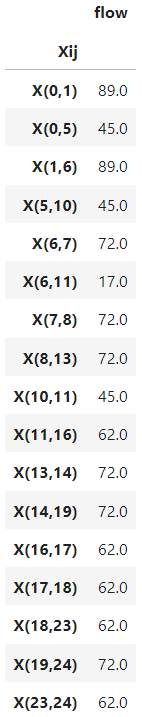
\includegraphics[width=0.13\linewidth]{flow1.png}}
  \hfill
  \subfigure{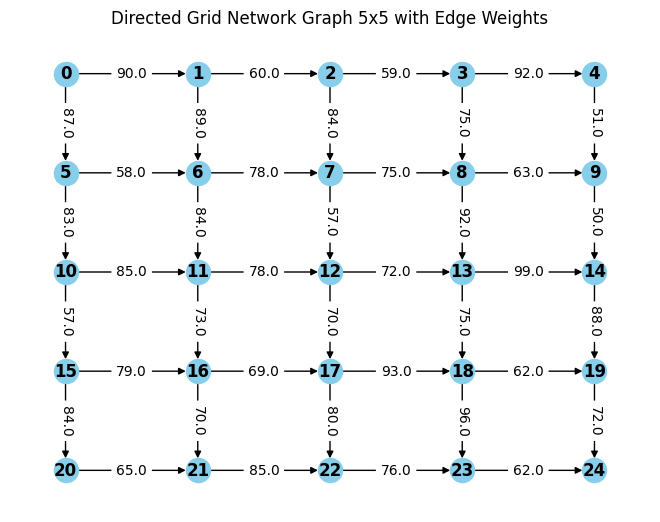
\includegraphics[width=0.8\linewidth]{5x5.png}}
  \caption{Đối với Network Graph}
\end{figure}
\newpage
\subsubsection{Phân tích độ hiểu quả của thuật toán}
\subsubsubsection{Độ phức tạp của thuật toán Successive Shortest Path}
{Thuật toán Dijkstra có độ phức tạp là $O((V+E)∗logV)$. ($V$ là số đỉnh, $E$ là cạnh)}

{Thuật toán Fulkerson: nếu trọng số trên đồ thị đều là số nguyên và giá trị tại nguồn cũng là số nguyên nên thuật toán sẽ kết thúc (nếu là giá trị vô tỉ thì thuật toán sẽ không thể dừng). Giả sử luồng tại vị trí nguồn có giá trị là $F$, mỗi lần tăng cường luồng thì giá trị tăng cường bé nhất là 1. Giả sử trong trường hợp xấu nhất, ta phải thực hiện $F$ lần thao tác tăng cường luồng để bài toán kết thúc (không xét đến trường hợp thuật toán kết thúc trước vì không tìm được luồng cực đại). Đối với thao tác cập nhập lại đồ thị, ta duyệt theo đường đi tìm được, nên trường hợp xấu nhất là có $V$ thao tác (với $V$ là số đỉnh đồ thị). Chung quy lại ta có độ phức tạp trong trường hợp xấu nhất là $
O(F.V)$.}

{Thuật toán algorithm 1: sử dụng ý tưởng kết hợp từ 2 thuật toán trên nên có độ phức tạp là: $O((V+E)∗logV + F.V)$}
\subsubsubsection{Thuật toán Cycle Cancelling để giải quyết cùng vấn đề }
{Ý tưởng chung của thuật toán: Tìm các luồng flow để lượng flow đi qua đồ thị đạt giá trị cực đại. Đổi chiều, dịch chuyển các lượng flow để giải cost bằng cách tăng cường luồng thông qua các chu trình âm. Đến khi không còn chu trình âm nữa thì giải thuật dừng lại, ta thu được đường đi với max-flow và min-cost. }
\newpage
{Mã giả:}
\begin{mdframed}
[hidealllines=true,backgroundcolor=gray!10]
\begin{lstlisting}
Establish a feasible flow x in the network
while ( GX contains a negative cycle ) do
    identify a negative cycle W
    ctth
    augment  units of flow along the cycle W
    update GX
\end{lstlisting}
\end{mdframed}
{Độ phức tạp của thuật toán:}

{Tìm các luồng để đạt được max-flow cho đồ thị có độ phức tạp $O(EF)$ với ($O(E)$ để tìm luồng tăng cường, $O(F)$ để tăng cường luồng). }

{Quá trình tìm kiếm chu trình âm có độ phức tạp là $O(E.V)$ nếu sử dụng thuật toán Bellman-Ford. (với $E$ là số cạnh, $V$ là số đỉnh của đồ thị) }

{Tổng lượng cost qua các flow lúc ban đầu không thể vượt quá $CPE$ (với $C$ và $P$ lần lượt là trọng số cost và capacity lớn nhất, $E$ là số đỉnh). Mỗi lần giảm cost dọc theo chu trình âm với lượng tối đa là 1. Trong trường hợp xấu nhất có tới $CPE$ thao tác.}

{Vậy độ phức tạp chung của giải thuật là $O(E^3.F.V.C.P)$}
\subsubsubsection{So sánh Runtime và Memory giữa Successive Shortest Path và Cycle Cancelling }
\textbf{So sánh trên Normal Graph}

\begin{figure}[h]
    \centering
    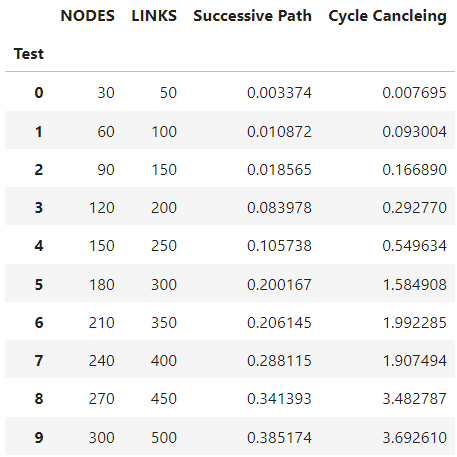
\includegraphics[scale=0.9]{runtime_normal.png}
    \caption{Thời gian chạy (đơn vị: $s$) của 2 chương trình với số nodes và links tăng dần:}
    \label{fig:enter-label}
\end{figure}
\newpage
{Có thể thấy rằng Successive Shortest Path có thời gian chạy tốt hơn nhiều so với Cycle Cancelling. Điều này được thể hiện rõ khi ta phân tích độ phức tạp của 2 thuật toán. Cycle Cancelling phải tốn rất nhiều chi phí cho việc tìm kiếm chu trình âm, trong khi Successive Shortest Path lại có thời gian chạy tốt hơn nhiều khi sử dụng Dijkstra. }

\begin{figure}[h]
    \centering
    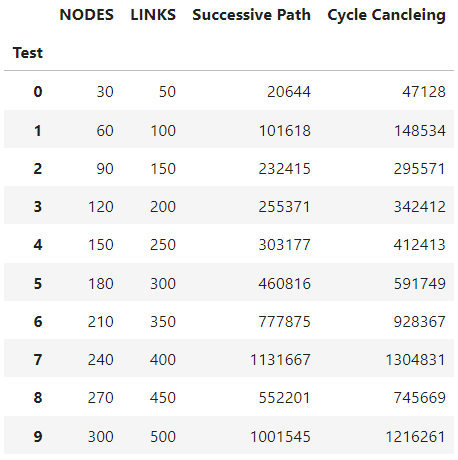
\includegraphics{memory_normal.png}
    \caption{Bộ nhớ (đơn vị: $byte$) đã sử dụng của 2 chương trình}
    \label{fig:enter-label}
\end{figure}

{Ta nhận thấy không có sự khác nhau quá lớn giữa memory của 2 thuật toán. Đa phần là Successive Shortest Path chiếm ít bộ nhớ hơn. Điều này có thể được lí giải do quá tình tìm kiếm chu trình âm trong Cycle Cancelling tốn nhiều chi phí hơn.}
\newpage
\textbf{So sánh trên Network Graph}
\begin{figure}[h]
  \centering
  \subfigure{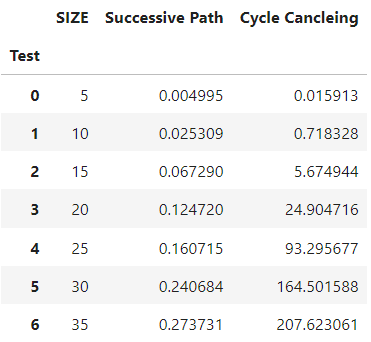
\includegraphics[width=0.45\linewidth]{runtime_grid.png}}
  \hfill
  \subfigure{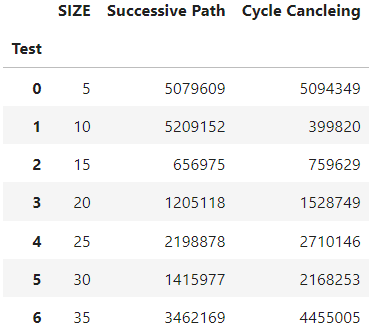
\includegraphics[width=0.45\linewidth]{memory_grid.png}}
  \caption{Thời gian chạy (đơn vị: $s$) và bộ nhớ (đơn vị: $byte$) đã sử dụng của 2 chương trình}
\end{figure}

{Ta có thể nhận thấy sự khác biệt rất lớn giữa thời gian chạy của 2 giải thuật. Giải thuật Successive Shortest Path nhanh hơn Cycle Canceling rất nhiều. Xét về bộ nhớ thì 2 thì successive shortest path xử dụng ít hơn cycle cancelling, nhưng nhìn chung cả 2 không có quá nhiều sự khác biệt. }

\newpage
\begin{thebibliography}{2}
\bibitem{doc1}
Thuật toán Mincost flow algorithm: \url{https://www.topcoder.com/thrive/articles/Minimum%20Cost%20Flow%20Part%20Two:%20Algorithms}
\bibitem{doc2}
Thuật toán Successive Shortest Path: \url{https://cp-algorithms.com/graph/min_cost_flow.html}
\bibitem{doc3}
Thuật toán Ford Fulkerson: \url{https://youtu.be/LdOnanfc5TM?si=1_PROuy1IEc_YZlN }
\bibitem{doc4}
Luồng cực đại trên đồ thị: \url{https://vnoi.info/wiki/algo/graph-theory/flow?fbclid=IwAR0RVmBo90OXy4ODZM0tycAZpslCZyU5MTuRse_SE2veir-7FRhqWta47Ek}
\bibitem{doc5}
Thuật toán Cycle Cancellinm: \url{https://hyperskill.org/learn/step/28463}
\bibitem{doc6}
Python cơ bản: \url{https://www.w3schools.com/}
\bibitem{doc7}
Thư viện NetworkX Python: \url{https://networkx.org/documentation/stable/tutorial.html 
Thư viện GAMSPy Python: GAMSPy User Guide — GAMSpy 0.11.3 documentation}
\bibitem{doc8}
A. Shapiro, D. Dentcheva, and A. Ruszczynski, \emph{Lectures on stochastic programming: modeling
and theory}. SIAM, 2021.
\bibitem{doc9}
Li Wang, \emph{A two-stage stochastic programming framework for evacuation planning in
disaster responses},  China

\end{thebibliography}
\end{document}
